% https://de.overleaf.com/latex/templates/a-quick-guide-to-latex/fghqpfgnxggz

\documentclass[10pt]{article}
% ========== Packages ==========
\usepackage[a4paper,
  left=10mm,
  right=10mm,
  top=10mm,
  bottom=17mm
]{geometry}

% \usepackage[ngerman]{babel} %Ändert die Sprache
\usepackage[T1]{fontenc} %Wichtig für ä ö ü
\usepackage{amssymb,amsmath,amsthm,amsfonts}
\usepackage{graphicx}
\usepackage{fancyhdr}
\usepackage[utf8]{inputenc}
\usepackage{multicol,multirow}
\usepackage{longtable} %Für lange Tabellen
\usepackage{arydshln} %Für gestrichelte Linien in Tabellen
\usepackage{tabularx}
\usepackage{pdfpages} %Zum einfügen von PDF's
\usepackage{hyperref} %Für hyperlinks
\hypersetup{bookmarks=true}
\usepackage{parskip}
\usepackage{caption} %Für die Beschriftung von Bilder
\captionsetup{justification=centering}
\captionsetup{font=it}
\setlength{\parindent}{0pt}
\usepackage{subcaption} %Für die Beschriftung unterteilter Bilder
\usepackage{float}
\floatstyle{plaintop}
\restylefloat{table}
\usepackage{siunitx}%Für einheiten im Symbolverzeichnis
% \usepackage[symbols,nogroupskip,sort=none]{glossaries-extra}%Für Symbolverzeichnis
% % \input{symbolverzeichnis}
\usepackage{lipsum}%Für pseudo text



\makeatletter %Für römische Zahlen
\newcommand*{\rom}[1]{\expandafter\@slowromancap\romannumeral #1@}

%Für die dicken Linien in Tabellen
\def\thickhline{%
  \noalign{\ifnum0=`}\fi\hrule \@height \thickarrayrulewidth \futurelet
   \reserved@a\@xthickhline}
\def\@xthickhline{\ifx\reserved@a\thickhline
               \vskip\doublerulesep
               \vskip-\thickarrayrulewidth
               \fi
      \ifnum0=`{\fi}}
\makeatother
\newlength{\thickarrayrulewidth}
\setlength{\thickarrayrulewidth}{2\arrayrulewidth}

%Sorgt dafür, dass nicht immer alles auf die ganze Seite verteilt wird.
\raggedbottom

% ========== Header and Footer ==========
\pagestyle{fancy}
\fancyhf{}
% \fancyhead[RE,LO]{Seite \thepage}
% \fancyhead[LE,RO]{\nouppercase{\leftmark}}
\fancyfoot[RE,LO]{Page \thepage}
\renewcommand{\headrulewidth}{0pt}
\renewcommand{\footrulewidth}{.5pt}

%Eigens erstellte Variablen
\newcommand{\plotWidth}{0.7}
\newcommand{\garphWidth}{0.7}
\newcommand{\linienAbstand}{2ex}
\newcommand{\linienDicke}{0.5pt}
\newcommand{\linienDickeDick}{1.5pt}


% \usepackage{calc}
% \usepackage{ifthen}
% \ifthenelse{\lengthtest { \paperwidth = 11in}}
%     { \geometry{top=.5in,left=.5in,right=.5in,bottom=.5in} }
% 	{\ifthenelse{ \lengthtest{ \paperwidth = 297mm}}
% 		{\geometry{top=1cm,left=1cm,right=1cm,bottom=1cm} }
% 		{\geometry{top=1cm,left=1cm,right=1cm,bottom=1cm} }
% 	}
% \pagestyle{empty}
\makeatletter
\renewcommand{\section}{\@startsection{section}{1}{0mm}%
                                {-1ex plus -.5ex minus -.2ex}%
                                {0.5ex plus .2ex}%x
                                {\normalfont\large\bfseries}}
\renewcommand{\subsection}{\@startsection{subsection}{2}{0mm}%
                                {-1explus -.5ex minus -.2ex}%
                                {0.5ex plus .2ex}%
                                {\normalfont\normalsize\bfseries}}
\renewcommand{\subsubsection}{\@startsection{subsubsection}{3}{0mm}%
                                {-1ex plus -.5ex minus -.2ex}%
                                {1ex plus .2ex}%
                                {\normalfont\small\bfseries}}
\makeatother
\setcounter{secnumdepth}{0}
\setlength{\parindent}{0pt}
\setlength{\parskip}{0pt plus 0.5ex}
% -----------------------------------------------------------------------


\begin{document}
\footnotesize

\begin{center}
\Large{\textbf{Applied Statistics and Data Analysis}} \\
\end{center}
\begin{multicols*}{2}
\setlength{\premulticols}{1pt}
\setlength{\postmulticols}{1pt}
\setlength{\multicolsep}{1pt}
\setlength{\columnsep}{2pt}


% Part I
\part{Statistical Process and Quality Control}
\section{Introduction}
\noindent\rule[\linienAbstand]{\linewidth}{\linienDickeDick}

\subsection{What is Statistical Quality and Process Control}
\noindent\rule[\linienAbstand]{\linewidth}{\linienDicke}
\textbf{Definition of Quality}\\
\begin{itemize}
  \item Quality means fitness for use. and
  \item Quality is inversely proportional to variability.
  \item My definition: Something is of quality if \emph{Is} and \emph{should} are the same.
\end{itemize}

\textbf{Statistical Process Control (SPC)}\\
Statistical process control is commonly understood as a way to optimise production and manufacturing processes.\\

\textbf{The Magnificent Seven}\\
The magnificent seven are the following seven statistical (graphical) methods for analysing data:
\begin{enumerate}
  \item histogram
  \item check sheet
  \item Pareto chart
  \item defect concentration diagram
  \item cause-and-effect diagram
  \item control chart
  \item scatter diagram
\end{enumerate}

\textbf{Check Sheet}\\
The check sheet is a simple method of quality control. As a rule, it consists of a ready-made form to register and count possible problems in a production process.\\
\begin{table}[H]
  \scriptsize
  \centering
  \begin{tabular}{l|cccc|l}
    causes            & \multicolumn{4}{l|}{interruptions/quarter} &  \\
                      & 1. & 2. & 3. & 4. & total \\ \hline
    drop phone        & 1  & 0  & 0 & 2  & 3\\
    battery empty     & 3  & 3  & 2 & 4  & 12\\
    driving in tunnel & 12 & 10 & 13 & 9 & 44\\
    press button      & 1  & 1  & 0  & 3 & 5\\
    accident          & 1  & 0  & 0  & 0 & 1\\
    phone broken      & 1  & 0  & 2  & 1 & 4\\
    no obvious reason & 3  & 4  & 3  & 5 & 15
  \end{tabular}
\end{table}

\textbf{Pareto Chart}\\
The Pareto chart is a special histogram, which is used to apply the causes of a problem in function from the greatest to the least serious. It is a statistical tool for visualizing the 80-20 principle.
\begin{figure}[H]
  \centering
  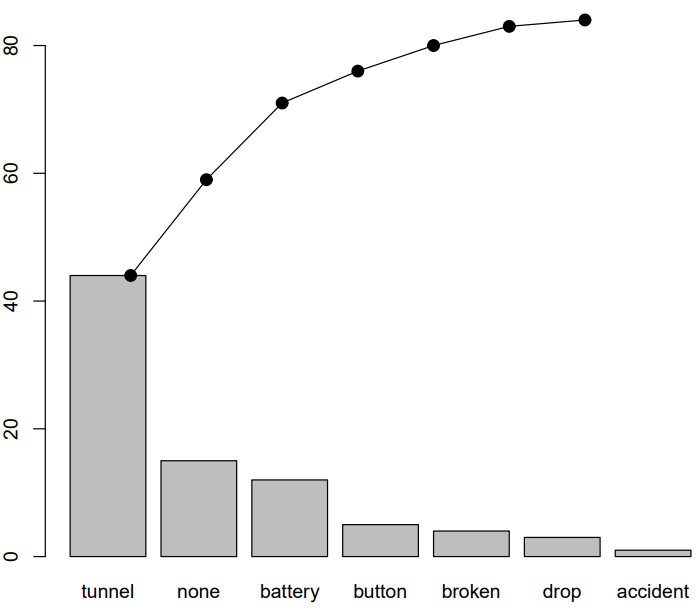
\includegraphics[width = 0.4\linewidth]{Pics/1.2.2.png}
  \caption{Pareto chart.}
\end{figure}

\textbf{Defect Concentration Diagram, Location Plot}\\
The graphical counterpart to the check sheet is the defect concentration diagram or the location plot. The diagram is used to graphically visualise the locations of the various defects on a physical object.
\begin{figure}[H]
  \centering
  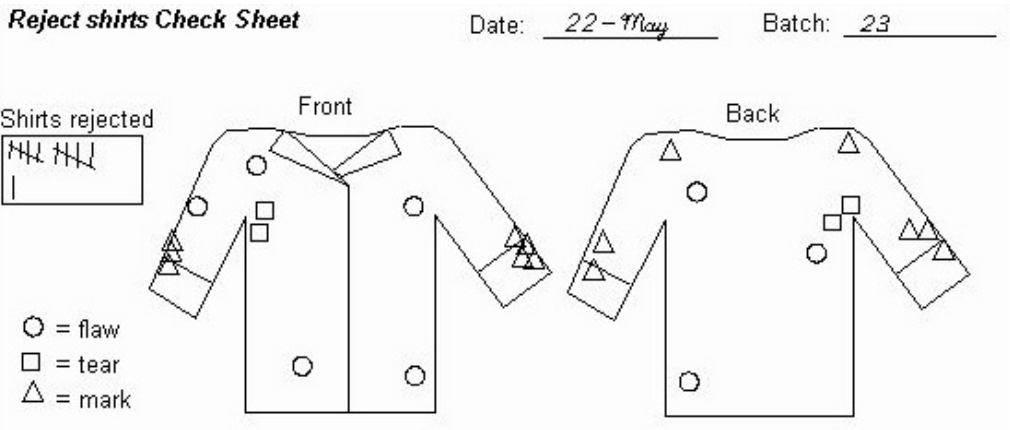
\includegraphics[width = 0.6\linewidth]{Pics/1.2.3.png}
  \caption{Defect concentration diagram or location plot: The locations of the various defects in the quality control of shirts are marked.}
\end{figure}

\textbf{Cause-and-Effect Diagram}\\
The cause-and-effect diagram is a tool in the form of a fishbone for the systematic identification of causes which make problems.
\begin{figure}[H]
  \centering
  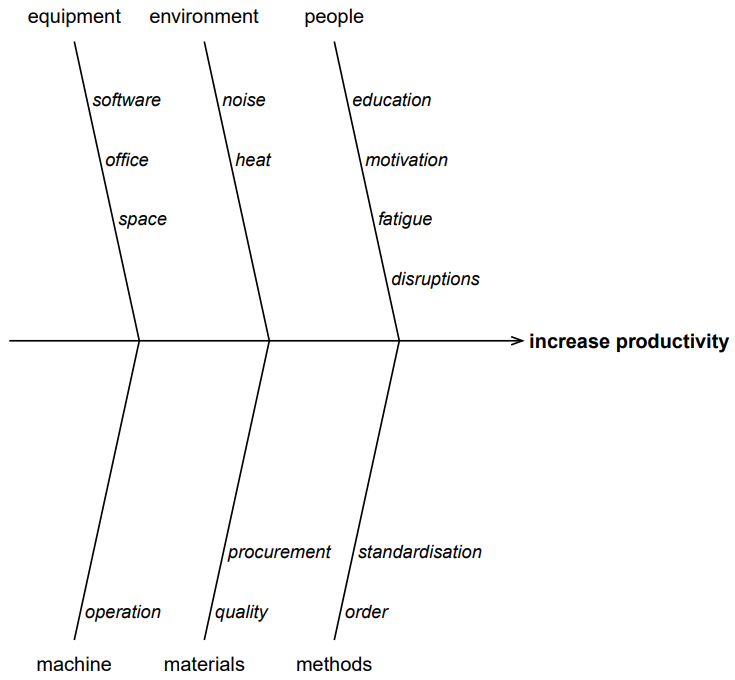
\includegraphics[width = 0.4\linewidth]{Pics/1.2.4.png}
  \caption{Cause-and-effect diagram.}
\end{figure}

\section{Control Charts}
\noindent\rule[\linienAbstand]{\linewidth}{\linienDickeDick}

\subsection{Control Charts versus Hypothesis Testing}
\noindent\rule[\linienAbstand]{\linewidth}{\linienDicke}
\begin{equation}
  \bar{X} \approx \mathcal{N}\left(\mu, \frac{\sigma^{2}}{n}\right)
\end{equation}

% Hypothesis:
% \begin{equation}
%   \begin{split}
%     H_0:& mu = mu_0 (Null-Hypothesis)\\
%     H_1:& mu \neq mu_0 (Alternative-Hypothesis)
%   \end{split}
% \end{equation}


\textbf{Arithmetic mean}
\begin{equation}
  \bar{x} = \frac{1}{n} \sum_{i=1}^n x_i
\end{equation}

Question: is $\left|\bar{x} - \mu_0\right|$ significant
- $\mu_0$ target value\\
- $\bar{x}$ Arithmetic mean of the measurements\\
Given: Level of significantce $\alpha$ = 0.0027

\subsection{The Control Chart}
\noindent\rule[\linienAbstand]{\linewidth}{\linienDicke}

\begin{figure}[H]
  \centering
  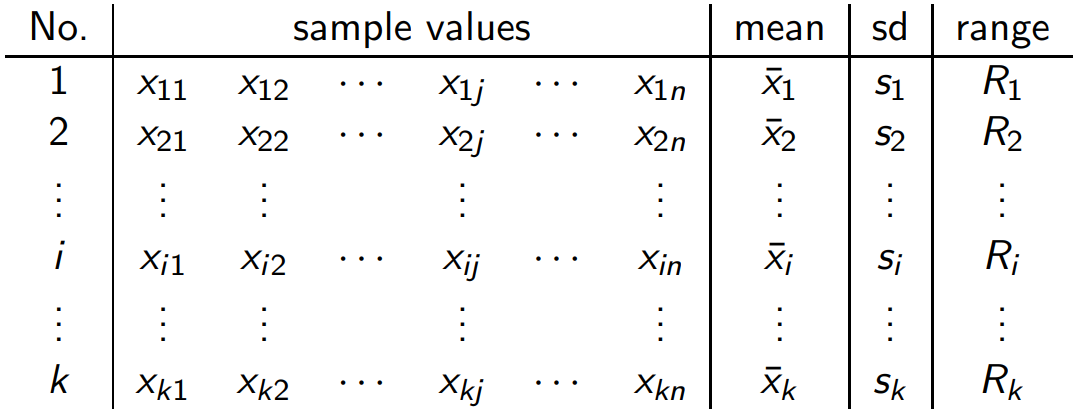
\includegraphics[width = 0.8\linewidth]{Pics/2.1.png}
  \caption{Data Set with Mean, Standard Deviation and Range}
  \label{2.1}
\end{figure}

\textbf{Mean values}
\begin{equation}
  \bar{x}_i = \frac{1}{n} \sum_{j=1}^n x_{ij}
\end{equation}

\textbf{Standard deviations}
\begin{equation}
  s_i = \sqrt{\frac{1}{n-1} \sum_{j=1}^n \left(x_{ij} - \bar{x}_i\right)^2}
\end{equation}

\textbf{Ranges}
\begin{equation}
  R_i = max\left \{x_{ij} | j \in \left \{1,...,n\right \} \right \} - min\left \{x_{ij} | j \in \left \{1,...,n\right \} \right \}
\end{equation}
for all $i \in \left \{1,...,k\right \}$

\subsection{Control Chart with R and $\bar{x}$}
\noindent\rule[\linienAbstand]{\linewidth}{\linienDicke}

\paragraph{R Chart}\mbox{}\\
\textbf{Mean Range}
\begin{equation}
  \bar{R} = \frac{1}{k} \sum^k_{i=1} R_i
\end{equation}

\textbf{Control limits}
\begin{equation}
    UCL = D_4 \bar{R}; \;\;\;\;\; LCL = D_3 \bar{R}
\end{equation}

\paragraph{$\bar{x}$ Chart}\mbox{}\\
\textbf{Mean Range}
\begin{equation}
  \bar{R} = \frac{1}{k} \sum^k_{i=1} R_i
\end{equation}

\textbf{Control limits}
\begin{equation}
  \begin{split}
    UCL = \mu + 3 \frac{\sigma}{\sqrt{n}}; \;\;\;\;\;  LCL = \mu - 3 \frac{\sigma}{\sqrt{n}}
  \end{split}
\end{equation}
$\mu$: Process mean\\
$\sigma$: Process standard deviation\\
Problem: We don't know $\mu$ and $\sigma$ so we have to estimate them:\\
We know that for an independent sample $x_1, ... ,x_n$ from a normal distribution with parameters $\mu$ and $\sigma$ the mean
\begin{equation}
  \bar{x} = \frac{1}{n} \sum_{j=1}^n x_{j}
\end{equation}
satisfies
\begin{equation}
  E\left(\bar{x}\right) = \mu \;\;\;\; and \;\;\;\; Var\left(\bar{x}\right) = \frac{\sigma^2}{n}
\end{equation}

The mean is an unbiased estimator with the standard error
\begin{equation}
  SE\left(\bar{x}\right) = \frac{\sigma}{\sqrt{n}}
\end{equation}

Assumption: R chart is under statistical control.\\
- The value $\bar{R}$ is a reliable estimate for the mean range.\\
- The value $\bar{R}$ is a reliable estimate for the process standard deviation
\begin{equation}
  \hat{\sigma} = \frac{\bar{R}}{d_2}
\end{equation}

Any samples excluded for construction of the R chart should also be disregarded for construction of the $\bar{x}$ chart.
This results in a sample of $k^\star$ valid samples, (where $k^\star$ denotes the reduced number of samples).
Mean values of $\bar{x}_1, ... ,\bar{x}_{k^\star}$ provide an estimate of $\mu$, i.e
\begin{equation}
  \hat{\mu} = \bar{\bar{x}} = \frac{1}{k^\star} \sum^{k^\star}_{i=1} \bar{x_i}
\end{equation}

\textbf{Control limits}
\begin{equation}
  \begin{split}
    UCL =& \bar{\bar{x}} + 3\frac{\bar{R}}{d_2} \frac{1}{\sqrt{n}}\approx \bar{\bar{x}} + A_2 \bar{R}\\
    UCL =& \bar{\bar{x}} - 3\frac{\bar{R}}{d_2} \frac{1}{\sqrt{n}}\approx \bar{\bar{x}} - A_2 \bar{R}
  \end{split}
\end{equation}

\subsection{Control Chart with $\bar{x}$ and s}
\noindent\rule[\linienAbstand]{\linewidth}{\linienDicke}

\paragraph{s Chart}\mbox{}\\
The centreline of the s chart is denoted by $\bar{s}$ and is calculated from the arithmetic mean of the standard deviations
\begin{equation}
  \bar{s} = \frac{1}{k} \sum^k_{i=1} s_i
\end{equation}

\textbf{Control limits}
\begin{equation}
    UCL = B_4 \bar{s}; \;\;\;\;\;  LCL = B_3 \bar{s}
\end{equation}

\paragraph{$\bar{x}$ Chart}\mbox{}\\
Using an s chart of a process that is under control, the process standard deviation can be estimated by
\begin{equation}
  \hat{\sigma} = \frac{\bar{s}}{c_4}
\end{equation}
Any samples excluded for construction of the s chart should also be disregarded for construction of the $\bar{x}$ chart.
This results in a sample of $k^\star$ valid samples, (where $k^\star$ denotes the reduced number of samples).
Mean values of $\bar{x}_1, ... ,\bar{x}_{k^\star}$ provide an estimate of $\mu$, i.e
\begin{equation}
  \hat{\mu} = \bar{\bar{x}} = \frac{1}{k^\star} \sum^{k^\star}_{i=1} \bar{x_i}
\end{equation}

\textbf{Control limits}
\begin{equation}
  \begin{split}
    UCL =& \bar{\bar{x}} + 3\frac{\bar{s}}{c_4} \frac{1}{\sqrt{n}} \approx \bar{\bar{x}} + A_3 \bar{s}\\
    UCL =& \bar{\bar{x}} - 3\frac{\bar{s}}{c_4} \frac{1}{\sqrt{n}} \approx \bar{\bar{x}} - A_3 \bar{s}
  \end{split}
\end{equation}

\subsection{Individual Control Charts}
\noindent\rule[\linienAbstand]{\linewidth}{\linienDicke}
Individual control charts have exactly one measurement per sample.
Problem: You cannot estimate variability from a single measurement.
Idea: Use variation of two adjacent measurements.
\textbf{Moving ranges}
\begin{equation}
  MR_i = |x_{i+1} - x_i|
\end{equation}
for all $i \in \left\{1,...,n-1\right\}$.

\textbf{Arithmetic mean of the moving ranges}
\begin{equation}
  \overline{MR} = \frac{1}{n-1} \sum_{i=1}^{n-1}MR_i
\end{equation}
\textbf{Estimated process standard deviation}
\begin{equation}
  \hat{\sigma} = \frac{\overline{MR}}{d_2} = \frac{\overline{MR}}{1.128}
\end{equation}
Since two neighboring measurements were used to calculate the moving ranges we have $d_2 = 1.128$.

\textbf{Centerline}
The centerline for the individuals control chart is the arithmetic mean of the measured values.
\begin{equation}
  \bar{x} = \frac{1}{k} \sum^k_{i=1} x_i
\end{equation}

\textbf{Control limits}
\begin{equation}
    UCL = \bar{x} + 3 \frac{\overline{MR}}{1.128}; \;\;\;\;\;  LCL = \overline{x} - 3 \frac{\overline{MR}}{1.128}
\end{equation}

\subsection{Control Charts for Attributes Data – p Chart}
\noindent\rule[\linienAbstand]{\linewidth}{\linienDicke}
Number of defectives under number tested is a discrete random variable.

Given: Random sample of size n, of which D parts are defective
We know: The number of defective D under n examined parts follows a binomial distribution with the unknown probability p of success.
\textbf{Estimated probability}
\begin{equation}
  \hat{p} = \frac{D}{n}
\end{equation}

\textbf{Variance}
\begin{equation}
  Var(\hat{p}) = \frac{p(1-p)}{n}
\end{equation}

\textbf{Given:}
- k random samples with $n_1,...,n_k$ values.
- Each of these samples contains $d_1,...,d_k$ defective products.
\textbf{k relative frequencies}
\begin{equation}
  p_1 = \frac{d_1}{n_1},...,p_k = \frac{d_k}{n_k}
\end{equation}

\textbf{Centerline}
The centreline and the control limits of a p chart are again
determined from a stable trial run with $k^\star$ valid samples.\\
Again $k^\star \leq k$ is the reduced number of samples.

Distinguish 2 cases:
1. The sample sizes $n_1,...,n_k$ are all equal to n.
2. The sample sizes are not all equal.

\paragraph{Case 1}\mbox{}\\
\textbf{Centerline}
\begin{equation}
  \bar{p} = \frac{1}{k^\star} \sum^{k^\star}_{i=1}p_i
\end{equation}
\textbf{Control limits}
\begin{equation}
  UCL = \bar{p} + 3\sqrt{\frac{\bar{p}(1-\bar{p})}{n}}; \;\;\;\;\; LSL = \bar{p} - 3\sqrt{\frac{\bar{p}(1-\bar{p})}{n}}
\end{equation}

\paragraph{Case 2}\mbox{}\\
\textbf{Centerline}
\begin{equation}
  \bar{p} = \frac{d_1 + \cdots + d_{k^\star}}{n_1 + \cdots + n_{k^\star}}
\end{equation}
\textbf{Control limits}
\begin{equation}
  UCL_i = \bar{p} + 3\sqrt{\frac{\bar{p}(1-\bar{p})}{n_i}}; \;\;\;\;\; LSL_i = \bar{p} - 3\sqrt{\frac{\bar{p}(1-\bar{p})}{n_i}}
\end{equation}
The control limits now depend on the index i.

\section{Statistical Properties of Control Charts}
\noindent\rule[\linienAbstand]{\linewidth}{\linienDickeDick}
Aim of process control using control charts: Keep the process under statistical control.
Or, if it is not at the beginning, to put it into statistical control by improving production conditions.

\subsection{Interpretation of Control Charts}
\noindent\rule[\linienAbstand]{\linewidth}{\linienDicke}

\paragraph{Western Electric Rules}
\begin{enumerate}
  \item Any single data point falls outside the limit defined by UCL and LCL (beyond the 3$\sigma$-limit).
  \item 2. Two out of three consecutive points fall beyond the limit defined by $\frac{2}{3}$ UCL and $\frac{2}{3}$ LCL on the same side of the centreline (beyond the 2$\sigma$-limit).
  \item Four out of five consecutive points fall beyond the limit defined by $\frac{1}{3}$UCL and $\frac{1}{3}$ LCL on the same side of the centreline (beyond the 2$\sigma$-limit).
  \item Nine consecutive points fall on the same side of the centreline (so-called run).
\end{enumerate}

\begin{table}[H]
  \setlength{\tabcolsep}{0.2em}
  \scriptsize
  \begin{tabular}{p{\linewidth / 2 - 0.5em}@{\hskip 1em}p{\linewidth / 2 - 0.5em}}
    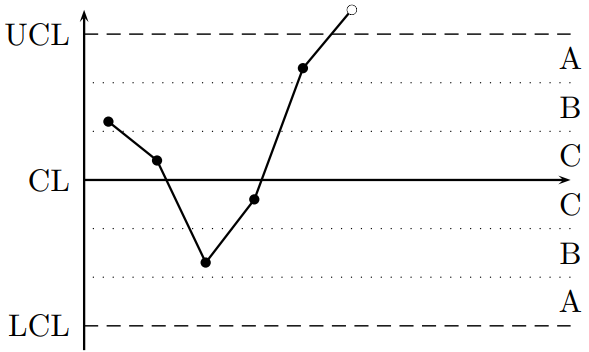
\includegraphics[width=\linewidth]{Pics/3.1.1.png}& 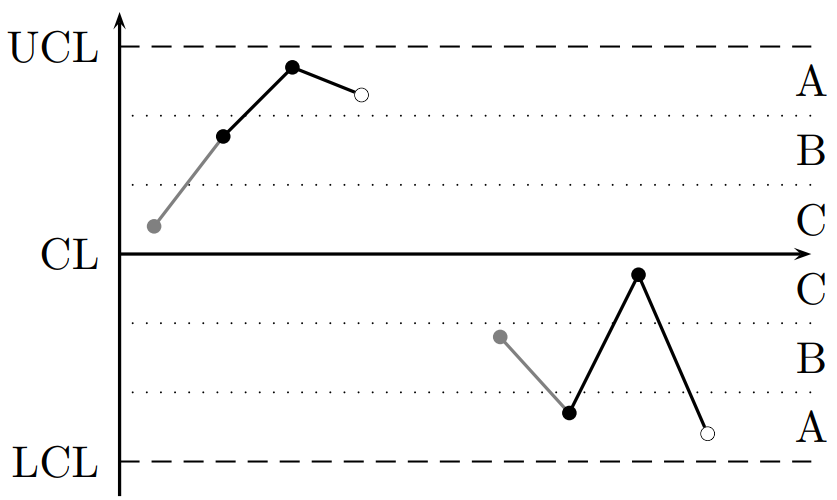
\includegraphics[width=\linewidth]{Pics/3.1.2.png} \\
    Rule 1: Any point beyond zone A. &
    Rule 2: Two out of three consecutive points fall on the same side in zone A or beyond.\\
    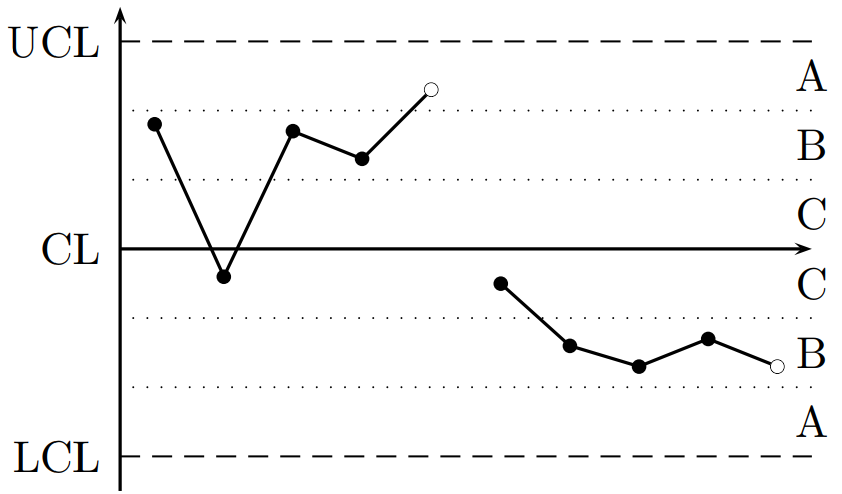
\includegraphics[width=\linewidth]{Pics/3.1.3.png}& 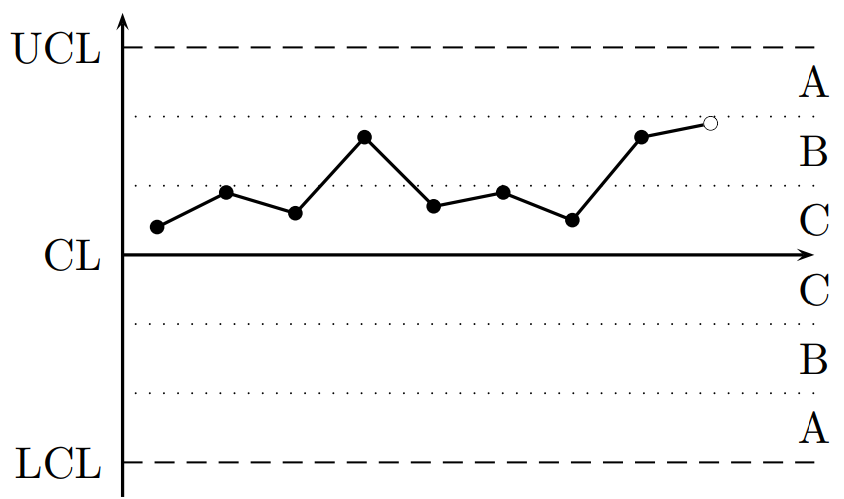
\includegraphics[width=\linewidth]{Pics/3.1.4.png} \\
    Rule 3: Four out of five consecutive points fall on the same side in zone B or beyond. &
    Rule 4: Nine consecutive points fall on the same side of the centreline.
  \end{tabular}
\end{table}

\subsection{Type I Error and Type II Error}
\noindent\rule[\linienAbstand]{\linewidth}{\linienDicke}
When monitoring a production process with a control chart, as with any statistical test, there are two wrong decisions possible.
\begin{equation}
  \begin{split}
    H_0:& \mu_0 = \mu \text{ i.e. process is not disturbed}\\
    H_1:& \mu_0 \neq \mu \text{ i.e. process is disturbed, } \mu_1 \text{ is true}
  \end{split}
\end{equation}
Denoted by:\\
 - $\mu_0$ the target value of the process\\
 - $\mu$ the considered statistic, eg. $\mu = \bar{x}$ or $\mu = R$\\
 - $\mu_1$ the true value of the considered statistic.\\

\textbf{Two wrong decisions possible:}\\
 - If a true null hypothesis $H_0$ is rejected we make a type I error. An intervention in the process is necessary, because the control limits are exceeded, although the process is not disturbed. This is called a false alarm.\\
 - If a false null hypothesis $H_0$ is accepted we make a type II error. There is no intervention, since the control limits are not exceeded, although the process is disturbed. This is called an omitted alarm\\

\textbf{Type I Error}\\
\begin{table}[H]
  \setlength{\tabcolsep}{0.2em}
  \scriptsize
  \begin{tabular}{p{\linewidth / 2 - 0.5em}@{\hskip 1em}p{\linewidth / 2 - 0.5em}}
    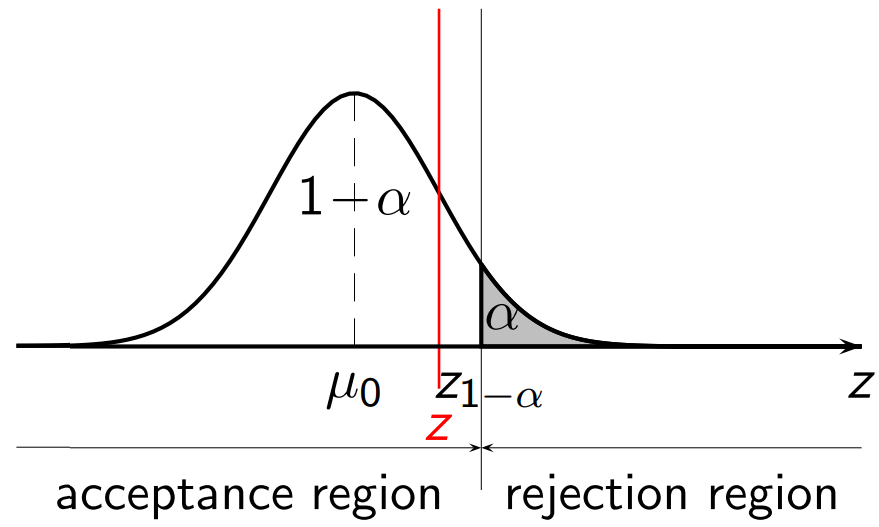
\includegraphics[width=\linewidth]{Pics/3.2.1.png}& 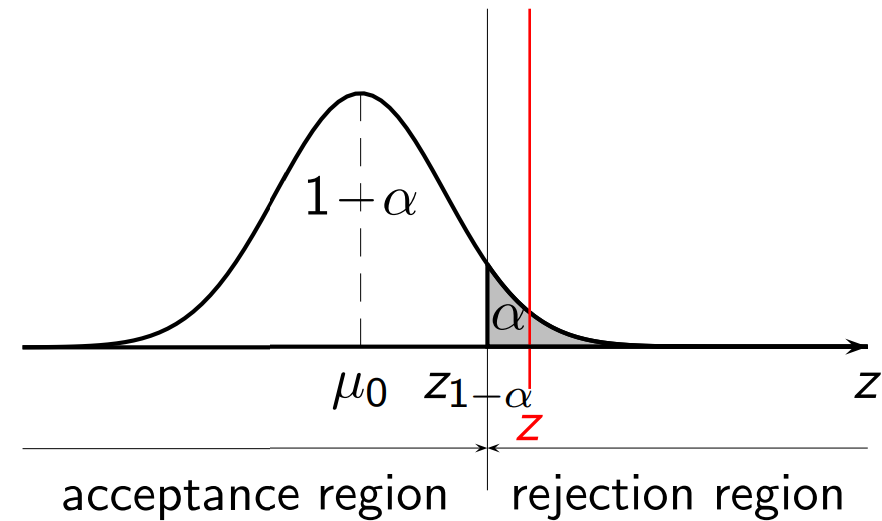
\includegraphics[width=\linewidth]{Pics/3.2.2.png} \\
    Let $h_0$ be true: Since $z < z_{1-\alpha}$ the null hypothesis is accepted. This is the right decision, which is made with probability $1-\alpha$. &
    Let $h_0$ be true: Since $z \geq z_{1-\alpha}$ the null hypothesis is rejected. This is the wrong decision (type I error), which is made with probability $\alpha$.
  \end{tabular}
\end{table}

\textbf{Type II Error}\\
\begin{table}[H]
  \setlength{\tabcolsep}{0.0em}
  \scriptsize
  \begin{tabular}{p{\linewidth / 2 - 0.5em}@{\hskip 1em}p{\linewidth / 2 - 0.5em}}
    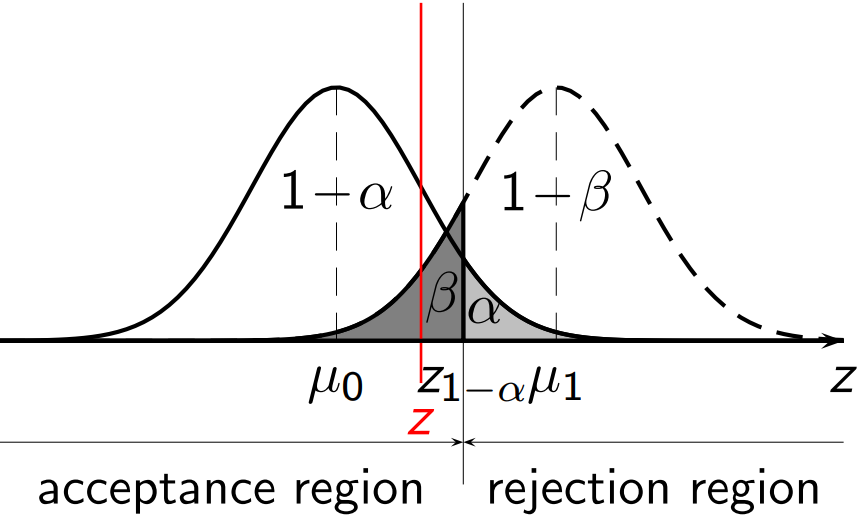
\includegraphics[width=\linewidth]{Pics/3.2.3.png}& 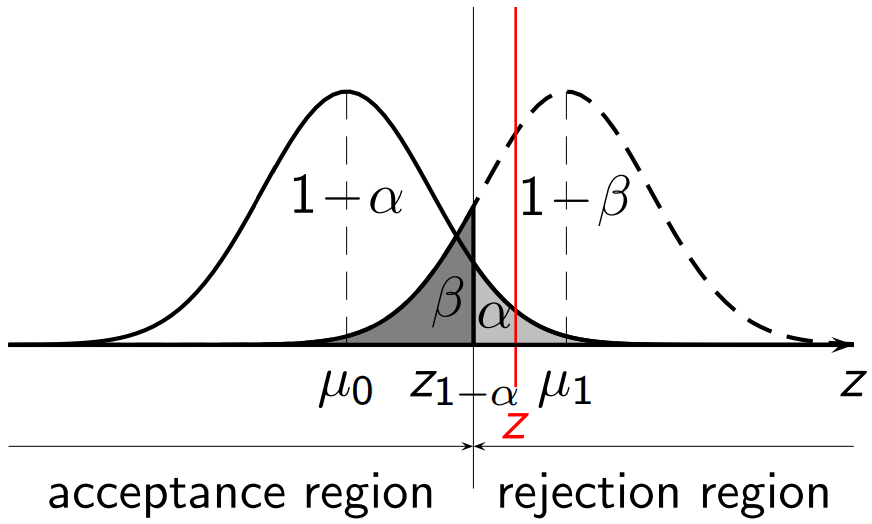
\includegraphics[width=\linewidth]{Pics/3.2.4.png} \\
    Let $H_0$ be false, $H_1$ true, i.e. the dashed density is true: Since $z < z_1-\alpha$ the null hypothesis is accepted. This is the wrong decision (type II error), which is made with probability $\beta$. &
    Let $H_0$ be false, $H_1$ true, i.e. the dashed density is true: Since $z \geq z_1-\alpha$ the null hypothesis is rejected. This is the correct decision, which is made with probability $1 - \beta$ (power).
  \end{tabular}
\end{table}

\subsection{Power Function and Operating Characteristic}
\noindent\rule[\linienAbstand]{\linewidth}{\linienDicke}
The power of a hypothesis test is the probability $1-\beta$ that the test correctly rejects the null hypothesis when the alternative hypothesis is true, i.e.
\begin{equation}
  \text{power} = P(\text{reject } H_0 | H_1 \text{ is true}) = 1-\beta
\end{equation}

\textbf{Power function}\\
Probability to reject the null hypothesis $H_0$ if $\mu_1$ is true.\\
\begin{equation}
  \delta = \frac{\mu_1 - \mu_0}{\sigma},
\end{equation}
or $\mu_1 = \delta\sigma + \mu_0$.\\
The variable $\delta$ is a normalized measure for the deviation of the disturbed from the undisturbed process in units of $\sigma$.\\
In statistical process control the power function is denoted by
\begin{equation}
  g(\mu_1) = g(\delta\sigma + \mu_0) = \tilde{g} (\delta).
\end{equation}
It is a measure for the probability of an intervention in the process.\\

 \textbf{Undisturbed Process}\\
 For an undisturbed process, i.e. $\mu = \mu_0$, we have
 \begin{equation}
   g(\mu_1) = \tilde{g} (0) = \alpha.
   \label{eq:3.3.a}
 \end{equation}

\textbf{Disturbed Process}\\
For a disturbed process we have
\begin{equation}
  \tilde{g}(\delta) = \Phi(\delta\sqrt{n} - z_q, 0, 1) + \Phi(-\delta\sqrt{n} - z_q, 0, 1)
  \label{eq:3.3.d}
\end{equation}
with $\Phi$ being
\begin{equation}
  \Phi(x, \mu, \sigma^2) = \frac{1}{\sqrt{2\pi\sigma^2}}\int^x_{-\infty}e^{-\frac{{(z-\mu)}^2}{2\sigma^2}}dz
\end{equation}


\subsection{Average Run Length}
\noindent\rule[\linienAbstand]{\linewidth}{\linienDicke}
If the $i_{RL}$-th sample is the first to result in an intervention, i.e. this sample is beyond the control limits, then $i_{RL}$ is called the run length of the control chart.\\
The ARL is the expected value of the probability i.e. the likelihood of exceeding the control limits when performing a test.
\begin{equation}
  ARL(\delta) = \frac{1}{p(\mu)} = \frac{1}{g(\mu_1)} = \frac{1}{\tilde{g}(\delta)}
\end{equation}

\textbf{Undisturbed Process}\\
If we have an undisturbed process with $\mu_1 = \mu_0$, i.e. with $\delta = 0$, then it follows from equation \ref{eq:3.3.a} that
\begin{equation}
  ARL(0) = \frac{1}{\alpha}.
\end{equation}

\textbf{Disturbed Process}\\
To determine the average run length of a disturbed process with $\mu = \mu_1$, i.e. $\sigma = \frac{\mu_1 - \mu_0}{\sigma}$ we use the power function $\tilde{g}(\delta)$ from equation \ref{eq:3.3.d}.

\subsection{Process Capability}
\noindent\rule[\linienAbstand]{\linewidth}{\linienDicke}
The specification limit (SL) is defined by
\begin{equation}
  SL = \frac{USL + LSL}{2}
\end{equation}

This performance is measured with so-called capability process ratios (PCR). The simplest process capability index is
\begin{equation}
  C_p = \frac{USL - LSL}{6\sigma}
\end{equation}
The capability process ratio $C_p$ expresses the ratio of the width of the tolerance range to the width of the process range.

\begin{itemize}
  \item $C_p = 1$ implies a reject rate of $\alpha \cdot 100\% = 0.27\%$.
  \item $C_p < 1$ implies a reject rate of more than $\alpha \cdot 100\% = 0.27\%$, i.e. the process capability is not guaranteed.
  \item $C_p > 1$ implies a reject rate of less than $\alpha \cdot 100\% = 0.27\%$,i.e. the process capability is guaranteed.

\end{itemize}

\section{Control Charts with Memory}
\noindent\rule[\linienAbstand]{\linewidth}{\linienDickeDick}

\textbf{Classical Shewhart control charts}\\
 - Decision to interfere with the manufacturing process is based on the result of the current sample.\\
 - No consideration of the development of the manufacturing process in the past (except with western electric rules).\\

\textbf{Modern control charts}\\
 - have a memory.

\textbf{Idea}\\
Linear combination of mean values $\bar{x}_j$ of samples from the past
\begin{equation}
 y_i = \alpha_i + \sum_{j=1}^i \beta_j \bar{x}_j,
\end{equation}
where $\alpha_i$ and the weights $\beta_1, ..., \beta_i$ can be arbitrary real numbers where the sum of all $\beta s = 1$.\\
Depending on how the weights are chosen, we get another type of control chart.

\subsection{CUSUM - Cumulative Sum Control Chart}
\noindent\rule[\linienAbstand]{\linewidth}{\linienDicke}
The CUSUM chart plots the cumulative sums of deviations of measurement values from the target value.\\

\textbf{Recursive procedure}\\
Using two statistics $C^+$, resp. $C^-$ the CUSUM chart sums up deviations above, resp. below the target value
\begin{equation}
  \begin{split}
    C^+_i &= max\{0, \bar{x}_i - (\mu_0 + K) + C_{i-1}^+\},\\
    C^-_i &= max\{0, (\mu_0 - K) - \bar{x}_i + C_{i-1}^+\}.
  \end{split}
\end{equation}
$C^+$ and $C^-$ only sum up deviations from the target value, which are greater than the reference value $K$.
The starting values of the recursion are $C^+ = 0$ and $C^- = 0$.\\

If a shift of $\Delta$ is to be detected then set
\begin{equation}
  K = \frac{\Delta}{2}.
\end{equation}
The constant $K$ is called reference value.\\

If the process is under controll the expected values of the statistic are both 0.\\
If the process is not under control, then the statistic sums up the deviations. If the sum of de deviations ($C^+$ and $C^-$) exceed the decision intercal $H$, then we should stop the process and look for the cause.\\

Rule of thumb for choosing the constants $K$ and $H$:
Let $\hat{\sigma}$ be an estimate for the process standard deviation.
- reference value = $K \frac{\hat{\sigma}}{2}$
- decision interval $H = 5\hat{\sigma}$

\begin{figure}[H]
  \centering
  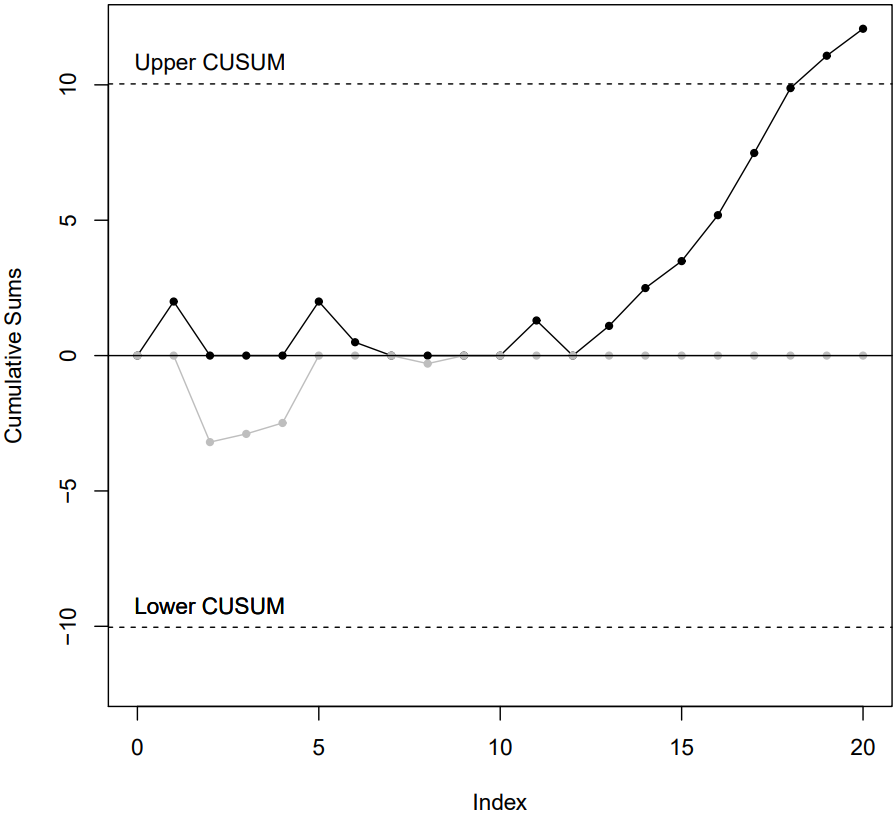
\includegraphics[width=0.8\linewidth]{Pics/4.1.png}
  \caption{CUSUM-Chart}
  \label{CUSUM}
\end{figure}


\subsection{EWMA - Exponentially Weighted Moving Average}
\noindent\rule[\linienAbstand]{\linewidth}{\linienDicke}
\textbf{Idea}\\
 - Monitoring means.\\
 - Wheights $\beta_j$ decay exponentially.\\

\textbf{Smoothing parameter $\lambda$}\\
Lambda lays between 0 and 1. The smoothing parameter $\lambda$ determines the influence of the previous sample mean $\bar{x}_j$ on the statistic. The smaller $\lambda$, the more values $\bar{x}_j$ are used for the decision. For $\lambda = 1$ only one sample is used and we get the well-known Shewhart $\bar{x}$ chart.\\

\textbf{Weights}\\
\begin{equation}
  \begin{split}
    \alpha_i =& (1-\lambda)^1 \mu_0\\
    \beta_j =& \lambda(1-\lambda)^{i-j} \text{with } j \in \{1,2,...,i\}.
  \end{split}
\end{equation}

\textbf{Statistics}\\
\begin{equation}
  y_i = (1-\lambda)^i \mu_0 + \lambda \sum_{j=1}^i(1-\lambda)^{i-j}\bar{x}_j
\end{equation}
Start: $y_0 = \mu_0$\\

\textbf{The same with recursion}\\
\begin{equation}
  y_i = (1-\lambda)y_{i-1} + \lambda\bar{x}_j
\end{equation}

\textbf{Assumptions}\\
If the process is under control, then $\bar{x}_i$ comes from a normal distribution with the expected value $\mu_0$ and the standard deviation $\frac{\sigma}{\sqrt{n}}$.\\
The standard deviation is either known or can be estimated from data. The statistic $y_i$ is then also normally distributed with $E(y_i) = \mu_0$ and
\begin{equation}
  Var(y_i) = \frac{\lambda}{2-\lambda}(1-(1-\lambda)^{2i})\frac{\sigma^2}{n}
\end{equation}

\textbf{Control limits}\\
These assumptions lead to the $3\sigma$ control limits:
\begin{equation}
  \begin{split}
    UCL_i =& \mu_0 + 3 \sqrt{\frac{\lambda}{2-\lambda}\left(1-(1-\lambda)^{2i}\right)}\frac{\sigma}{\sqrt{n}}\\
    LCL_i =& \mu_0 - 3 \sqrt{\frac{\lambda}{2-\lambda}\left(1-(1-\lambda)^{2i}\right)}\frac{\sigma}{\sqrt{n}}
  \end{split}
\end{equation}

The asymtotic control limits are:
\begin{equation}
  \begin{split}
    UCL_i =& \mu_0 + 3 \sqrt{\frac{\lambda}{2-\lambda}}\frac{\sigma}{\sqrt{n}}\\
    LCL_i =& \mu_0 - 3 \sqrt{\frac{\lambda}{2-\lambda}}\frac{\sigma}{\sqrt{n}}
  \end{split}
\end{equation}

\textbf{Estimate of process standard error}\\
\begin{equation}
  \hat{\sigma} = \frac{\bar{s}}{c_4}
\end{equation}

\begin{figure}[H]
  \centering
  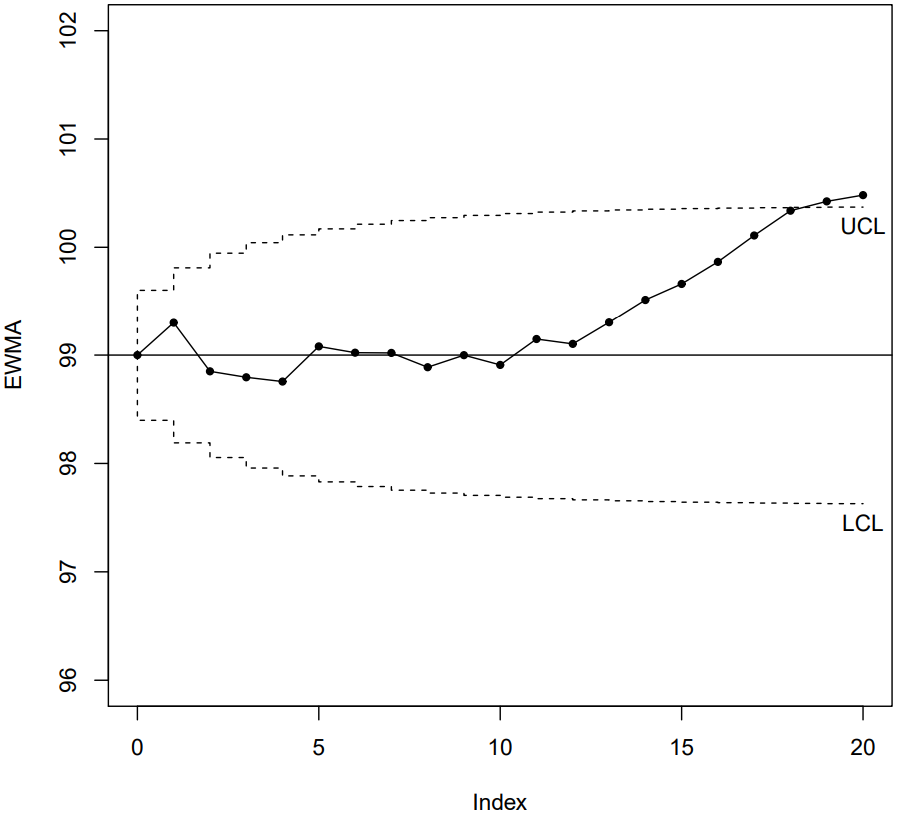
\includegraphics[width=0.8\linewidth]{Pics/4.2.png}
  \caption{EWMA-Chart}
  \label{EWMA}
\end{figure}

\section{Acceptance Sampling}
\noindent\rule[\linienAbstand]{\linewidth}{\linienDickeDick}
Acceptance control is based on acceptance sampling plans, which contain instructions based on which the acceptance or return of a lot is decided.\\
We should remember that the actual point of acceptance control is not to value quality, but to decide whether or not delivery will likely pass quality control.

\textbf{Idea:} Draw random samples from a lot and make a decision on the quality of the lot based on this information.

\subsection{Plans for Attributes}
\noindent\rule[\linienAbstand]{\linewidth}{\linienDicke}
\textbf{Percent defective}\\
We have a lot of N parts (known). The number of defective parts m (unknown) with $0 \leq m \leq N$ is observed. Thus, the percent defective is:
\begin{equation}
  p = \frac{m}{N}
\end{equation}

\textbf{Acceptance sampling plan} consitst of:\\
 - Sample size n,\\
 - the number of defective parts x in the sample, where $0 \leq x < n$,\\
 - the acceptance number c, where $0 \leq c < n$ and\\
 - the rule: if $x \leq c$, then the lot is accepted, if $x > c$, then the lot is rejected.\\

\textbf{Hypothesis test}\\
The rule above can also be formulated as a hypothesis test:
\begin{equation}
  \begin{split}
    H_0:& x \leq c,\text{ i.e. the lot is not rejected.}\\
    H_1:& x > c,\text{ i.e. the lot is rejected.}\\
  \end{split}
\end{equation}

As with any hypothesis test the following two errors can be made.\\

\textbf{Type I Error}\\
$H_0$ true, but rejected (Lot is good but is rejected)\\
Probability for this to happen (false negative): $\alpha$. (Producer's risk)\\
The producer wants to avoid type I error, i.e. does not want good lots to be returned.\\

\textbf{Type II Error}\\
$H_0$ false, but accepted (Lot is bad but is accepted)\\
Probability for this to happen (false positive): $\beta$. (Consumer's risk)\\
The consumer wants to avoid type II error, i.e. does not want to accept bad lots.\\


In an agreement between a producer and a consumer the following parameter must de defined:\\
- $\alpha$: The producer's acceptable probability of falsly rejecting a good lot,\\
- $\beta$: The consumer's acceptable probability of falsly accepting a bad lot,\\
- $p_{\alpha}$ the producer's minimal percentage defective needed for a lot to be returned (The producer does not want to take back lots with $p < p_{\alpha}$.),\\
- $p_{\beta}$ the consumer's maximal percentage defective needed for a lot to be accepted (The consumer wants to reject lots with $p_{\beta} < p$ whenever possible).

\subsection{Operating Characteristic}
\noindent\rule[\linienAbstand]{\linewidth}{\linienDicke}
The operating characteristic, short OC, is the probability of accepting a lot as a function of the percent defective p.\\
The number of defective units X is a hypergeometric random variable. There are N parts in total, among which m defective and N - m are good parts. So a sample of size n is drawn at once. The probability that among these n parts are at most c parts defective is given by
\begin{equation}
  OC(p) = P(X \leq c)= \sum^c_{k=0} P(X = k) = \sum^c_{k=0} \frac{\binom{pN}{k}\binom{N-pN}{n-k}}{\binom{N}{n}}
\end{equation}
For a given lot size N, the parameters n and c of the acceptance sampling plan determine the form of the OC curve.\\

\textbf{Ideal OC Curve}\\
If all parts of a lot get checked we get an ideal acceptance sampling plan:
\begin{figure}[H]
  \centering
  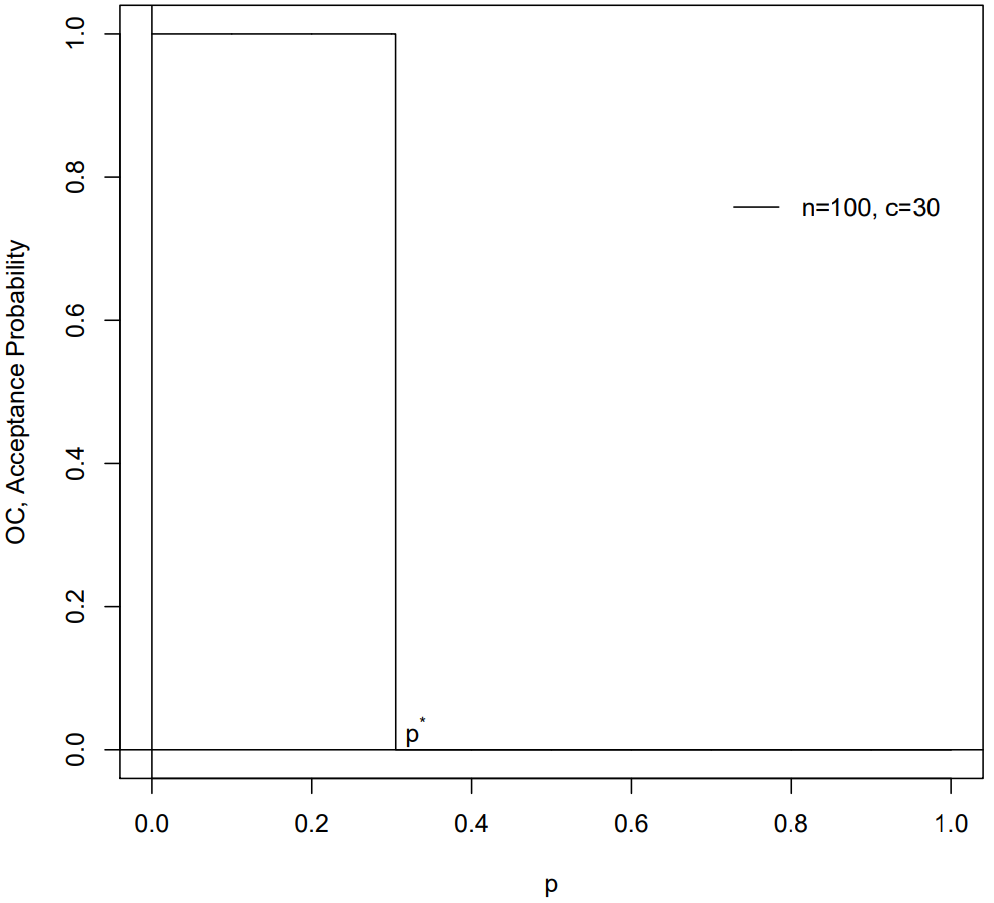
\includegraphics[width=0.8\linewidth]{Pics/5.1.1.png}
  \caption{OC curve of an ideal acceptance sampling plan}
\end{figure}

\textbf{OC Curves - Examples}
\begin{figure}[H]
  \centering
  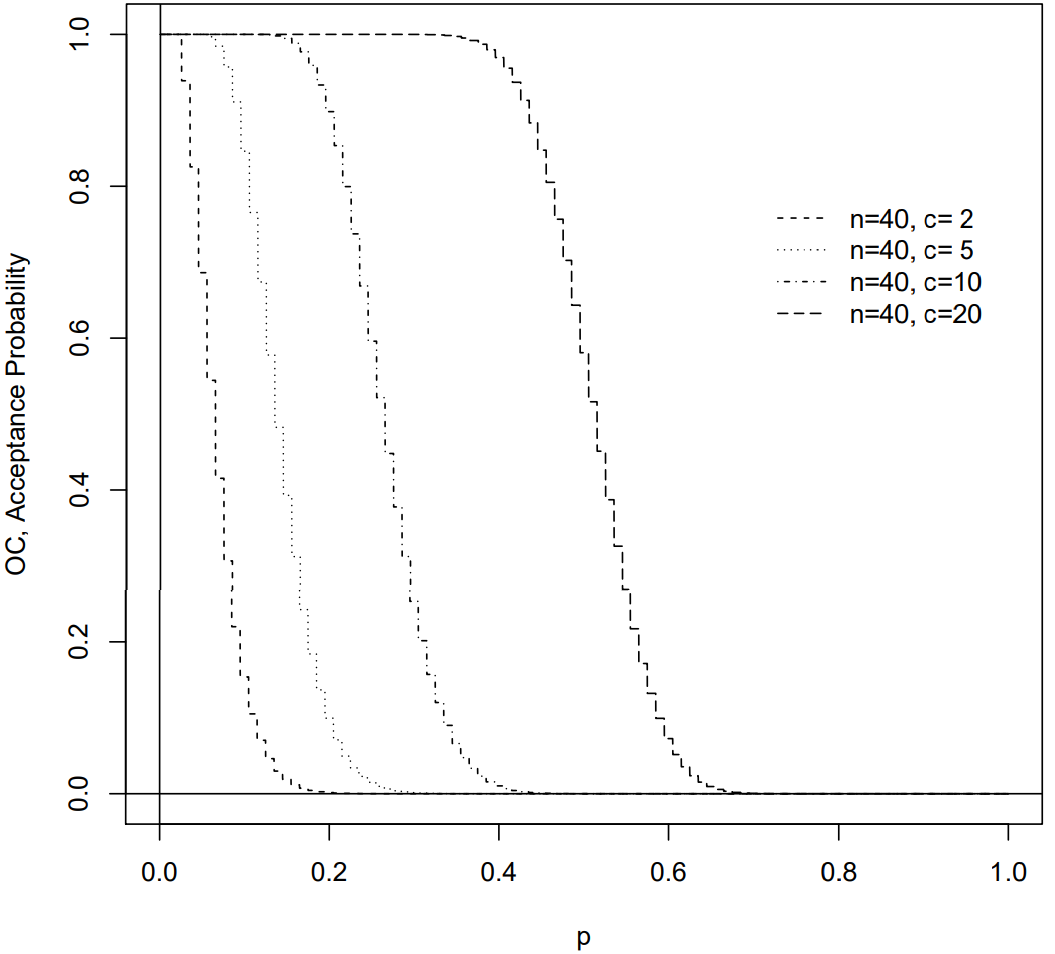
\includegraphics[width=0.8\linewidth]{Pics/5.1.2.png}
  \caption{OC curve with fixed n and increasing c}
\end{figure}

\begin{figure}[H]
  \centering
  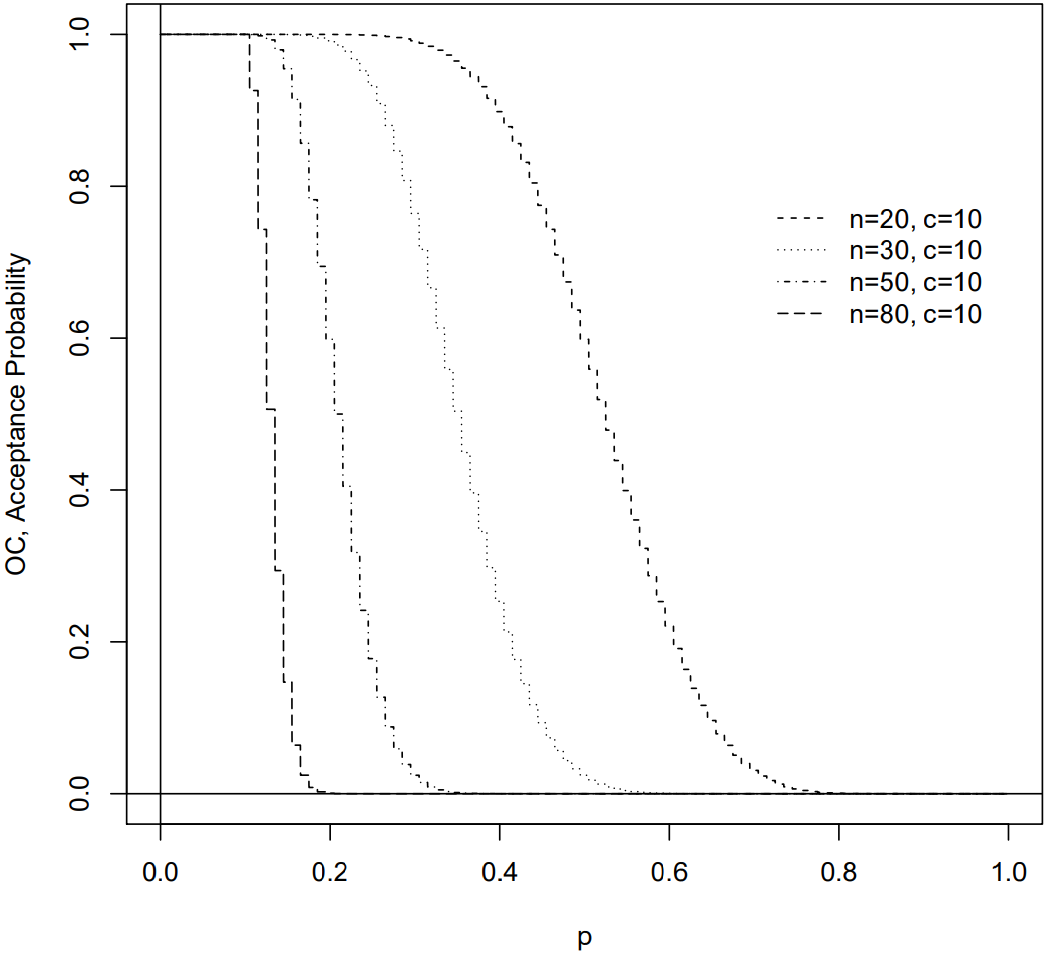
\includegraphics[width=0.8\linewidth]{Pics/5.1.3.png}
  \caption{OC curve with increasing n and fixed c}
\end{figure}

\subsection{Parameters of an Acceptance Sampling Plan}
\noindent\rule[\linienAbstand]{\linewidth}{\linienDicke}
n and c are to be chosen such that:\\
- n is as small as possible,\\
- the producer risk is at most equal to $\alpha$, i.e. $OC(p_{\alpha}) \leq 1 - \alpha$, and\\
- the consumer risk is at most equal to $\beta$, i.e. $OC(p_{\beta}) \geq \beta$\\

The pair $(p_{\alpha}, 1-\alpha)$ is called producer risk point and the pair $(p_{\beta}, \beta)$ is called consumer risk point.\\
n and c are calculated by brute force. The resulting OC curve is not a perfect fit since only integer values can be choosen.\\

\textbf{Real OC Curve}
\begin{figure}[H]
  \centering
  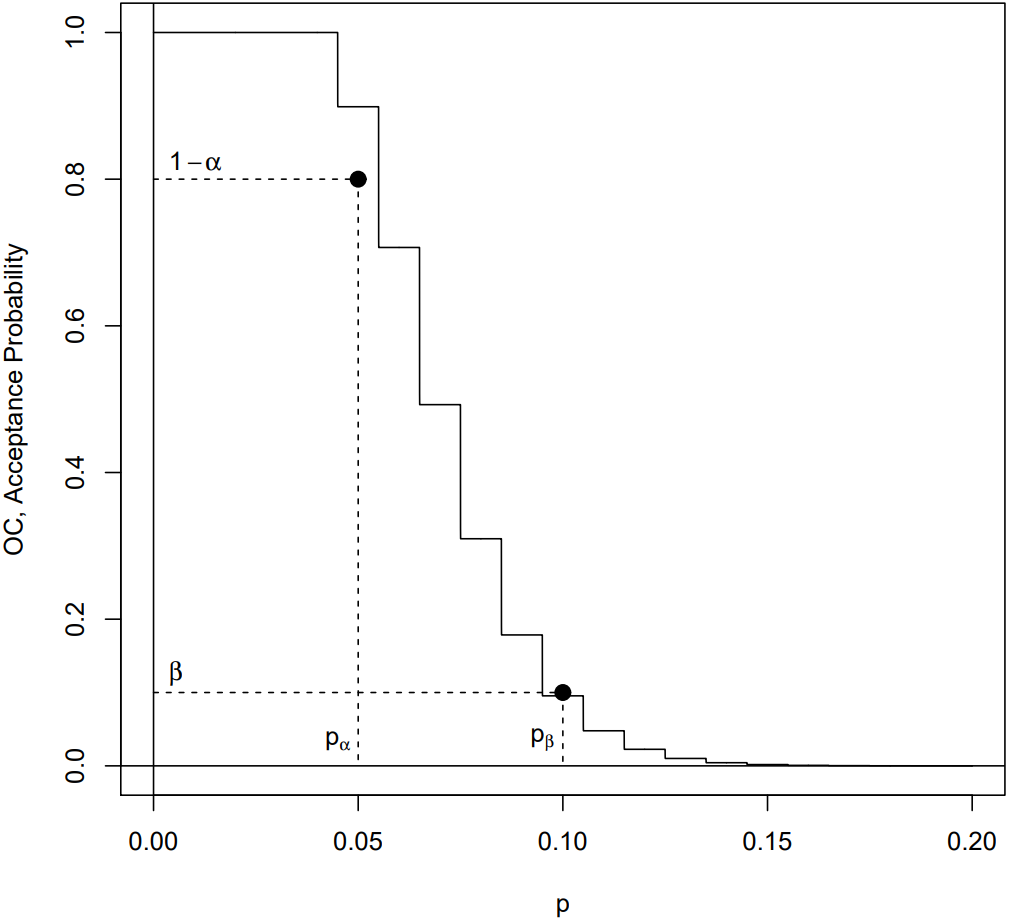
\includegraphics[width=0.8\linewidth]{Pics/5.1.4.png}
  \caption{OC curve of a real acceptance sampling plan.}
\end{figure}


\subsection{Acceptance Sampling Plans for Variables}
\noindent\rule[\linienAbstand]{\linewidth}{\linienDicke}
It is always possible to reduce an acceptance sampling plan for variables to an acceptance sampling plan for attributes by saying:\\

- If $LSL \leq x \leq USL$, then the part is fit for use.\\
- If $x < LSL \text{ or } USL < x$, then the part is rejected\\

By counting the number of rejected parts, we again have an acceptance sampling plan for attributes.


% Part II
\part{Multiple Regression}
\section{Simple Linear Regression}
\noindent\rule[\linienAbstand]{\linewidth}{\linienDickeDick}
One of the most important and widely used statistical technique is regression analysis. This is a statistical technique for investigating and modelling relationships between variables.

\subsection{Simple Linear Regression Model}
\noindent\rule[\linienAbstand]{\linewidth}{\linienDicke}
A simple linear regression model is a model with a single predictor variable that has a relationship with a response that is a straight line.\\

\textbf{Model}
\begin{equation}
  y = \beta_0 + \beta_1x \cdot \varepsilon
\end{equation}
where $\beta_0$ and $\beta_1$ are unknown and fixed parameters.\\

\textbf{Variables and error}\\
- Perdictor / input / explanatory variable x (deterministic)\\
- Response / output variable y (random variable)\\
- Uncorrelated random error $\varepsilon $ with
\begin{equation}
  E(\varepsilon ) = 0
\end{equation}
and unknown variance
\begin{equation}
  Var(\varepsilon ) = \sigma^2
\end{equation}
Since the error is a random value, y is also a random value.\\

\textbf{Aim}\\
Find Parameters $\hat{\beta}_0, \hat{\beta}_1$ and $\hat{\sigma}^2$ such that model fits data as well as possible.

\textbf{Assumptions}\\
The error $\varepsilon $ is normaly distributed:
\begin{equation}
  E \approx \mathcal{N}(0, \sigma^2) \Rightarrow E(y) = \beta_0 + \beta_1 x
\end{equation}

\subsection{Estimation of the Parameters}
\noindent\rule[\linienAbstand]{\linewidth}{\linienDicke}
\textbf{Method of least square}\\
Minimise:
\begin{equation}
  S(\beta_0, \beta_1) = \sum_{i=1}^n(y_i-(\beta_0 + \beta_1x_i))^2
\end{equation}

Calculating:
\begin{equation}
  \hat{\beta}_0 = \bar{y} - \hat{\beta}_1\bar{x} \;\;\text{with}\;\; \hat{\beta}_1 = \frac{S_{xy}}{S_{xx}}
\end{equation}
where
\begin{equation}
  S_{xx} =  \sum^n_{i=1}(x_i - \bar{x})^2 \;\;\text{and}\;\; S_{xy} =  \sum^n_{i=1}(x_i - \bar{x})(y_i - \bar{y})
\end{equation}
with
\begin{equation}
  \bar{x} = \frac{1}{n}\sum_{i=1}^n x_i  \;\;\text{and}\;\; \bar{y} = \frac{1}{n}\sum_{i=1}^n y_i
\end{equation}

\textbf{Residual}\\
The difference between the $i$th observed value $y_i$ and its fitted value $\hat{y_i}$ is the residual
\begin{equation}
  e_i = y_i - \hat{y}_i = y_i - (\beta_0 + \beta_1x_i)
\end{equation}

\textbf{Mean of residuals}\\
\begin{equation}
  \bar{e} = \frac{1}{n} \sum_{i=1}^n e_i = 0
\end{equation}

\textbf{Unbiased estimator}\\
An unbiased estimator $\hat{\sigma}^2$  is obtained from the error sum of squares
\begin{equation}
  \hat{\sigma}^2 = \frac{1}{n - 2} \sum_{i=1}^n (e_i - \bar{e})^2 = \frac{1}{n - 2} \sum_{i=1}^n e_i^2
\end{equation}
Notice that we have to divide by the degrees of freedom $n - 2$ to make the estimator unbiased. (2 because we have two parameters to find).\\

\textbf{Distribution of the estimators}\\
To be able to answer how well the model fits the data, whether the model can be used as a reliable predictor and whether the the assumptions of constant variance and uncorrelated errors are met, we need to know the distributions of the estimators $\beta_0$ and $\beta_1$.\\
Since the estimators $\beta_0$ and $\beta_1$ are calculated using the random variable $y$, the estimators themselves are random variables which follow the distributions
\begin{equation}
  \hat{\beta}_0 \sim \mathcal{N}\left(\beta_0, \sigma^2\left(\frac{1}{n} + \frac{\bar{x}^2}{S_{xx}}\right)\right)
\end{equation}
and
\begin{equation}
  \hat{\beta}_1 \sim \mathcal{N}\left(\beta_1, \frac{\sigma^2}{S_{xx}}\right).
\end{equation}

\subsection{Tests and Confidence Intervals}
\noindent\rule[\linienAbstand]{\linewidth}{\linienDicke}
In many cases we are not only interested in estimating the model parameters but also in testing hypothesis and constructing confidence intervals.\\

\paragraph{Statistical Test on the Slope}\mbox{}\\
\textbf{Hypothesis}
\begin{equation}
  \begin{split}
    H_0:& \beta_1 = \beta_{1,0}\\
    H_1:& \beta_1 \neq \beta_{1,0}
  \end{split}
\end{equation}
The null hypothesis states that the observations follow the model of simple linear regression with $\beta_{1} = \beta_{1.0}$ and arbitrary $\beta_0$ and $\sigma$. Where $\beta_{1.0}$ is the slope we want to test.\\

\textbf{Estimated standard error}\\
We can estimate the standard error with the error sum of squares.
\begin{equation}
  se(\hat{\beta}_1) = \sqrt{\frac{\hat{\sigma}^2}{S_{xx}}} \text{    with    } S_{xx} =  \sum^n_{i=1}(x_i - \bar{x})^2
\end{equation}

\textbf{Test statistic}
\begin{equation}
  T = \frac{\hat{\beta}_1 - \beta_{1,0}}{se(\hat{\beta}_1)}
\end{equation}
Under the null hypothesis the test statistic $T$ follows a Student’s t-distribution with $n - 2$ degrees of freedom. Values of t are usually found in a table.\\
If T is smaller than t (from the table), we accept the null hypothesis and conclude that the data agrees also with a model with the slope $\beta_{1,0}$.


\textbf{P-Value}\\
The probability, under the null hypothesis, of obtaining a result equal to or more extreme than what was actually estimated. If the value T of the test statistic is larger than the critival value t (from the table) the null hypothesis is not rejected i.e. it is plausible to assume that the data fits the model.

\paragraph{Confidence Test}\mbox{}\\
The test statistic
\begin{equation}
  T = \frac{\hat{\beta}_1 - \beta_{1,0}}{se(\beta_1)}
\end{equation}
is accepted on the significance level $\alpha$ if
\begin{equation}
  t_{\frac{\alpha}{2}, n-2} \leq T \leq t_{-\frac{\alpha}{2}, n-2}
\end{equation}



\textbf{Confidence interval on the slope}
\begin{equation}
  \hat{\beta}_1 - t_{\frac{\alpha}{2}, n-2} \cdot se(\beta_1) \leq \beta_1 \leq  \hat{\beta}_1 + t_{-\frac{\alpha}{2}, n-2} \cdot se(\beta_1)
\end{equation}
\begin{equation}
  \left[\hat{\beta}_1 - t_{\frac{\alpha}{2}, n-2} \cdot se(\beta_1), \hat{\beta}_1 - t_{-\frac{\alpha}{2}, n-2} \cdot se(\beta_1)\right]
\end{equation}

Interpretation:
The true value lies in the confidence interval with high probability.

\section{Residual Analysis}
\noindent\rule[\linienAbstand]{\linewidth}{\linienDickeDick}


\subsection{Introduction}
\noindent\rule[\linienAbstand]{\linewidth}{\linienDicke}
In our simple linear regression models we made the following assumptions:
\begin{enumerate}
  \item The relationship between response and the regressors is linear.
  \item The error $\varepsilon$ has mean zero.
  \item The error $\varepsilon$ has constant variance $\sigma^2$
  \item The errors are uncorrelated.
  \item The errors are normally distributed
\end{enumerate}
If some assumptions are violated we should be able to see them in the errors $\varepsilon_i$. On the other hand, the errors are unknown to us, so we have to deal with the residuals
\begin{equation}
  e_i = y_i - \hat{y}_i \;\;\;\text{for all}\;\;\; i \in {1,...,n}
\end{equation}
instead. The residuals are estimators of the random errors.\\

\textbf{Scaled Residuals}\\
If the errors are normally distributed, so are the residuals of a least-squares estimate. Since the variance of the residuals depends on $x_0$ it is not equal to the variance of the errors. Therefore we use scaled residuals
\begin{equation}
  \tilde{e}_i = \frac{e_i}{\sqrt{1 - \left(\frac{1}{n} + \frac{(x_i - \bar{x})^2}{S_{xx}}\right)}} \;\;\;\text{for all}\;\;\; i \in {1,...,n}
\end{equation}


\textbf{Coefficient of Determination}\\
The coefficient of determination is a measure of the linear relationship between the response variable and the fit.\\

In simple linear regression with only one explanatory variable the coefficient of determination is defined by
\begin{equation}
  R^2 = \frac{SS_{\textup{fit}}}{S_{yy}}
\end{equation}
where
\begin{equation}
  \begin{split}
    SS_{\textup{fit}} &= \sum_{i=1}^n(\hat{y}_i - \bar{\hat{y}}_i)^2 = \hat{\beta}_1^2 S_{xx}\\
    SS_{yy} &= \sum_{i=1}^n(y_i - \bar{y}_i)^2
  \end{split}
\end{equation}
Therefore the coefficient of determination is
\begin{equation}
  R^2 = \hat{\beta}_1^2 \frac{S_{xx}}{S_{yy}} = \frac{S_{xy}^2}{S_{xx} S_{yy}} = \textup{Cor}(x, y)^2
\end{equation}

In multiple regression and simple linear regression with at least one explanatory variable the coefficient of determination is identical to the squared correlation between the response variable $y$ and the fitted values $\hat{y}$
\begin{equation}
  R^2 = \textup{Cor}(y, \hat{y})^2 = \frac{S_{y\hat{y}}^2}{S_{yy} S_{\hat{y}\hat{y}}}
\end{equation}

The coefficient of determination is a global measure for the goodness of fit and it says nothing about the suitability of the regression model.

\subsection{Diagnostic Tools}
\noindent\rule[\linienAbstand]{\linewidth}{\linienDicke}

\textbf{Tukey-Anscombe Plot}

\section{Multiple Linear Regression}
\noindent\rule[\linienAbstand]{\linewidth}{\linienDickeDick}
A multiple regression model is a model which involves more than one regressor variable.\\

\subsection{Model and Estimation}
\noindent\rule[\linienAbstand]{\linewidth}{\linienDicke}
We generalise the concept of a simple linear regression model with only one explanatory variable to a multiple linear regression model
\begin{equation}
  y = \beta_0 + \beta_1 x_1 + \beta_2 x_2 + ... + \beta_m x_m +\varepsilon,
\end{equation}

$\beta_0$ is the intercept\\
$\beta_k$ is the slope in the $x_k$ direction for all $k \in {1, 2, ..., m}$.


\textbf{Least-Squares Estimation of the Regression Coefficient}\\
The general idea and philosophy of teh multiple linear regression modle are the same as in the simple linear regression model. To calculate the according factors the matrix notation is used.
\begin{equation}
  \mathbf{y} = \mathbf{X} \mathbf{\beta} + \varepsilon
\end{equation}

Aufg. 8.5.1 is important!!

\subsection{Diversity of Modelling Possibilities}
\noindent\rule[\linienAbstand]{\linewidth}{\linienDicke}

\textbf{Polynomial Regression}\\
If we want to use a polynomial of degree two to describe a relationship, then the model has the following form
\begin{equation}
  y = \beta_0 + \beta_1x + \beta_2 x^2 + \varepsilon
\end{equation}
If we define the new variables $\texttt{lin} = x$ and $\texttt{quad} = x^2$, then we obtain mathematically the same model
\begin{equation}
  y = \beta_0 + \beta_1 \cdot \texttt{lin} + \beta_2 \cdot \texttt{quad} + \varepsilon
\end{equation}
which is now a multiple linear regression model.

\textbf{Nonlinear Functions and Linear Regression}\\
Experience shows that in most real-world regression problems, the variables must be transformed to get the best results. Four examples:
\begin{itemize}
  \item Inverting the nonlinear equations
  \begin{equation}
    \begin{split}
      y =& \frac{1}{a+be^{-x}}\\
      y =& \frac{ax}{b+x}
    \end{split}
    \;\;\;\;\;\;
    \begin{split}
      \text{gives}\\
      \text{gives}
    \end{split}
    \;\;\;\;\;\;
    \begin{split}
      \frac{1}{y} =& a + be^{-x}\\
      \frac{1}{y} =& \frac{1}{a} + \frac{a}{b} \frac{1}{x}
    \end{split}
  \end{equation}
  \item Taking logarithms of the nonlinear equations
  \begin{equation}
    \begin{split}
        y &= ax^b\\
        y &= ax^{bg(x)}
    \end{split}
    \;\;\;\;\;\;
    \begin{split}
      \text{gives}\\
      \text{gives}
    \end{split}
    \;\;\;\;\;\;
    \begin{split}
      \textup{ln}(y) &= \textup{ln}(a) + b\textup{ln}(x)\\
      \textup{ln}(y) &= \textup{ln}(a) + bg(x)
    \end{split}
  \end{equation}
\end{itemize}
It is important to realise that also such transformations change the form of the error term. If we are not allowed to alter the original additive error term, then we need to use nonlinear least-squares regression.

\textbf{Binary Explanatory Variables}\\
In all our examples, the explanatory variables have been continuous so far. This is not necessary.\\
If the binary variable $x_b$ is the only variable in the model
\begin{equation}
  y = \beta_0 + \beta_1 x_b + \varepsilon
\end{equation}
then
\begin{equation}
  \begin{split}
    y =& \beta_0 + \varepsilon\\
    y =& \beta_0 + \beta_1 + \varepsilon
  \end{split}
  \;\;\;
  \begin{split}
    \textup{if}\; x_b = 0\\
    \textup{if}\; x_b = 1
  \end{split}
\end{equation}

\textbf{Factor Variables}\\
Explanatory variables can be strongly (linearly) correlated.
$\Rightarrow$difficult to interpret the results of the regression analysis and
should be avoided.





\textbf{Binary Explanatory Variables}\\
Variable is discrete with values 0 and 1.\\

Factor Variables

\section{Sensitivity and Robustness}
\noindent\rule[\linienAbstand]{\linewidth}{\linienDickeDick}

\subsection{Residual Analysis}
\noindent\rule[\linienAbstand]{\linewidth}{\linienDicke}
The graphical tools Tukey-Anscombe plot, scale-location plot and q-q plot which check goodness of fit for the simple linear regression model can also be used for multiple linear regression models.\\
In addition to the Tukey-Anscombe plots mentioned above the \emph{Residuals vs. Leverage plot} is introduced which will be discussed in the next section.\\

In multiple regression, it is no longer clear which explanatory variable might cause a deficit. To find out graphically, the residuals $e = y - \hat{y}$ are plotted versus an explanatory variable $x_k$ used as the horizontal axis instead of the fitted values $\hat{y}$.\\

\subsection{Influential Observations}
\noindent\rule[\linienAbstand]{\linewidth}{\linienDicke}
The answer to the question whether an observation is an outlier depends on the model. If outliers remain in the data, the question arises of how strongly they influence the analysis.\\
Influence diagnostics is based on the idea to remove one observation, repeat the analysis and measure the change. \textbf{Cook’s distance measure} is a very popular influence diagnostic tool which measures the change of the fitted values if one observation $i$ is omitted.
\begin{equation}
  d_i = \frac{(\hat{\textbf{y}}_{(-1)} - \hat{\textbf{y}})^t(\hat{\textbf{y}}_{(-1)}-\hat{\textbf{y}})}{p \hat{\sigma}^2}
\end{equation}
where $p = m + 1$ is the number of estimated parameters in the case of a model with intercept and $p = m$ in the case without intercept.\\
Fortunately it is not necessary to repeat the analysis $n$ times. A mathematical simplification leads to the equivalent form
\begin{equation}
  d_i = \frac{\tilde{e}_{std,i}^2}{p}\frac{h_{ii}}{1-h_{ii}}
\end{equation}
Cook’s distance measure is a function of the $i$th standardised residual $\tilde{e}_{std,i}$ and the so-called leverages $h_{ii}$ of the $i$th observation. The leverages
\begin{equation}
  h_{ii} = \textbf{H}_{ii} = (\textbf{X}(\textbf{X}^t\textbf{X})^{-1}\textbf{X}^t)_{ii}
\end{equation}
are the diagonal entries of the hat matrix $\textbf{H}$. Leverages $h_{ii}$ satisfy $0 \geq h_{ii} \geq 1$ and the mean of all leverages is always $\frac{p}{n}$.\\

Interpretation of leverages:
\begin{itemize}
  \item A large leverage $h_{ii}$ has a big influence on the fitted values.
  \item A large leverage $h_{ii}$ reduces the variance of the $i$th residual, and therefore the $i$th observation is close to regression line (hyper-plane).
  \item Leverage is a measure of how far away the explanatory values of an observation are from those of the other observations.
\end{itemize}

When is an observation a leverage point?\\
\textbf{Rule of thumb:} Observations are dangerous if\\
\begin{equation}
  h_{ii} > 2 \frac{p}{n}
\end{equation}

\textbf{Huber's classification:}\\ Observations with
\begin{itemize}
  \item $h_{ii} \leq 0.2$ are harmless.
  \item $ 0.2 < h_{ii} < 0.5$ are potentially dangerous.
  \item $0.5 < h_{ii}$ should be avoided.
\end{itemize}

\textbf{Rule of thumb for Cook's distance measure:}
\begin{itemize}
  \item If $d_i > 1$ then the ith observation is dangerous.
  \item If $d_i \leq 1$ then the ith observation is harmless.
\end{itemize}


\begin{table}[H]
  \setlength{\tabcolsep}{0.2em}
  \scriptsize
  \begin{tabular}{p{\linewidth / 2 - 0.5em}@{\hskip 1em}p{\linewidth / 2 - 0.5em}}
    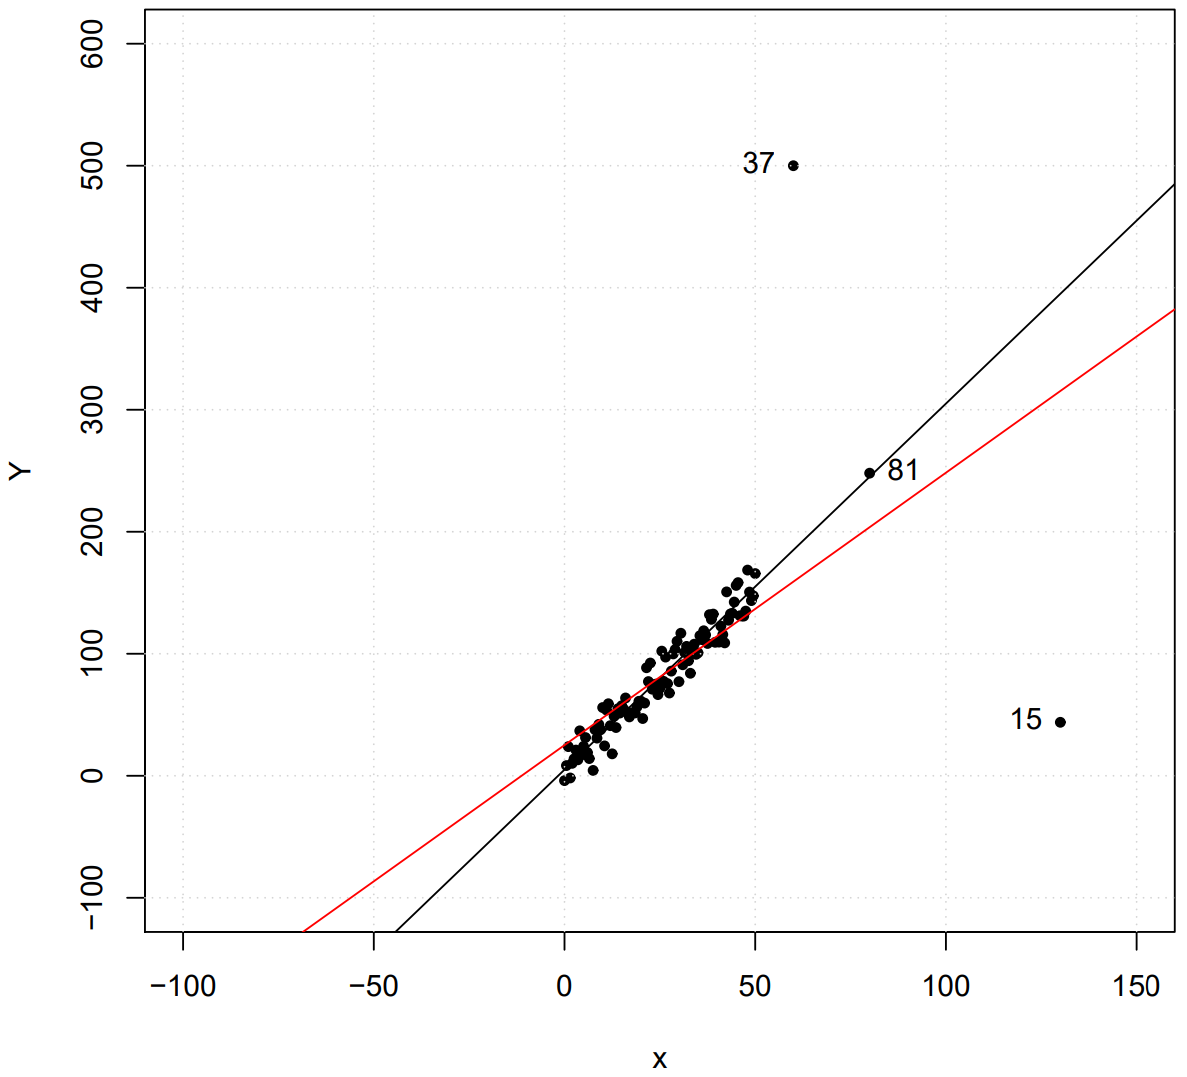
\includegraphics[width=\linewidth]{Pics/10.2.3.png}& 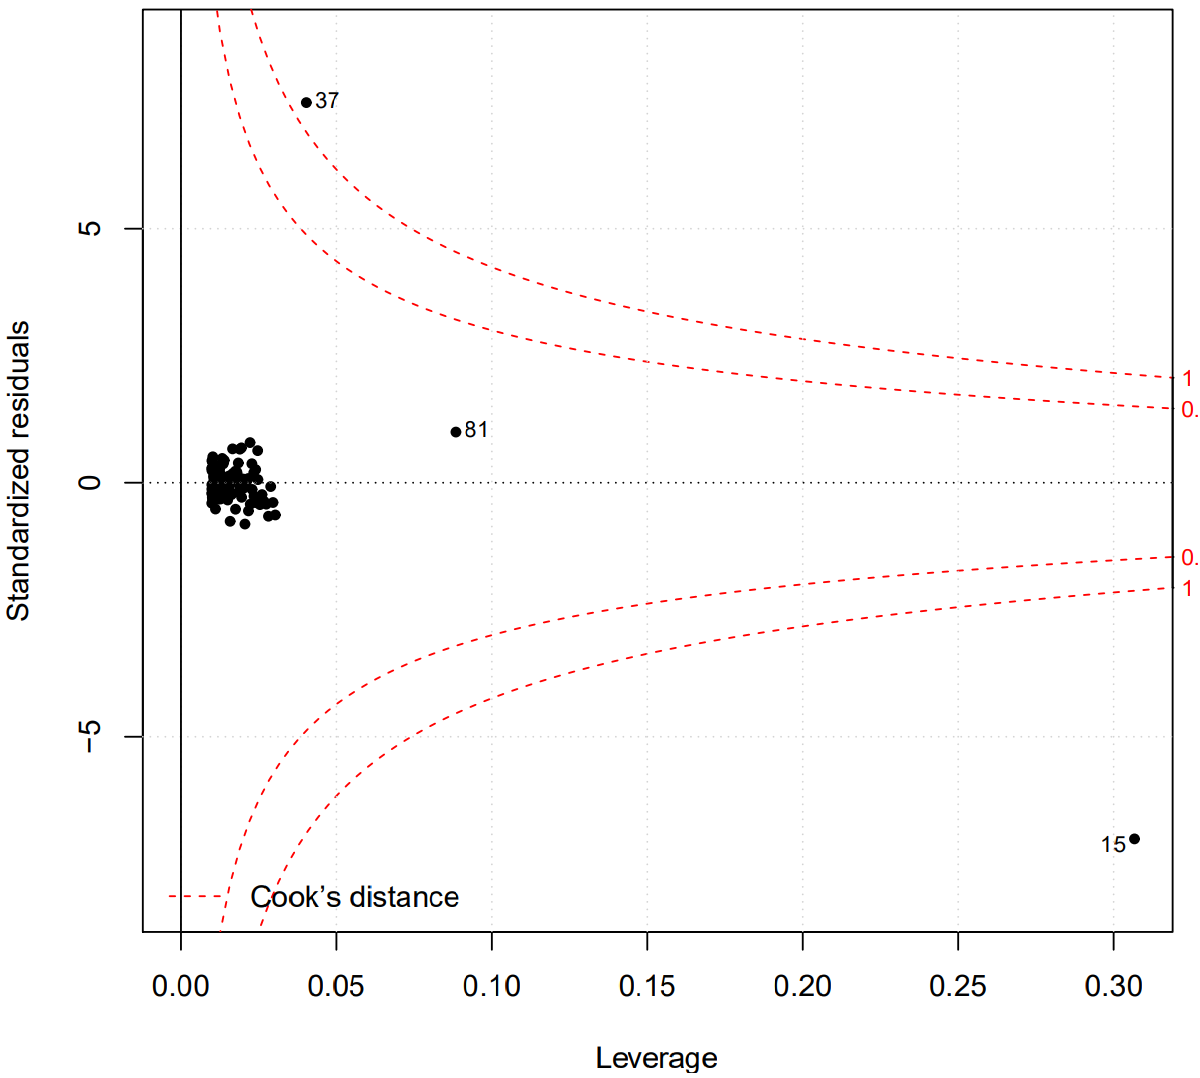
\includegraphics[width=\linewidth]{Pics/10.2.4.png} \\
    Artificial data with two outliers. Original model (black) and estimated best fit (red). &
    Standardised residuals versus leverages with two outliers. Contours of Cook’s distance measure (red).\\
  \end{tabular}
\end{table}

\subsection{Weighted linear regression}
\noindent\rule[\linienAbstand]{\linewidth}{\linienDicke}
It certainly makes sense to give greater weight to the observations with smaller random error. That is, the more precise observations gain weight in the statistical analysis.\\
Therefore we need to find the least-squares estimate for weighted multiple regression.\\
we want to find the vector of least-squares estimators $\beta$, which minimise

\begin{equation}
  S(\mathbf{\beta}) = \sum^n_{i = 1}w_i\varepsilon^2_i) = \varepsilon^t \mathbf{W} \varepsilon =
  (\mathbf{y}-\mathbf{X}\mathbf{\beta})^t \mathbf{W}(\mathbf{y}-\mathbf{X}\mathbf{\beta})
\end{equation}

which simplifies to the so-called weighted least-squares normal equations
\begin{equation}
  \mathbf{X}^t\mathbf{Wy} = \mathbf{X}^t\mathbf{WX}\hat{\pmb{\beta}}
\end{equation}

The solution of the normal equations is the least-squares estimator
\begin{equation}
  \hat{\pmb{\beta}} = (\mathbf{X}^t\mathbf{WX})^{-1} \mathbf{X}^t\mathbf{Wy}
\end{equation}


\subsection{Robust Methods}
\noindent\rule[\linienAbstand]{\linewidth}{\linienDicke}
The goal of robust statistics is to find parameter estimates as if the outliers did not exist\\

The robustness of an estimator can be investigated by two measures: the influence function and the breakdown point. Both measures are based on the idea of studying the effect of an estimator under the influence of gross errors, i.e. arbitrary added data.

\textbf{Breakdown Point}\\
The breakdown point is the minimal proportion of incorrect observations which cause completely unrealistic estimates.\\
\textbf{Gross Error Sensitivity}\\
The gross error sensitivity is based on the influence function and measures the maximum effect of a single observation on the estimated value.\\
\textbf{Robust Regression M-Estimator}\\
The influence of an outlier in observation $i$ is manifested in a large residual $e_i$. Therefore, the main idea of robust regression is to introduce weights $w_i$ which weigh down this influence. If we want to limit the influence of large residuals the function
\begin{equation}
  \Psi(e) = w_i e_i
\end{equation}
must be limited. This can be achieved, for instance by the Hubert's $\psi$ -function.
\begin{figure}[H]
  \centering
  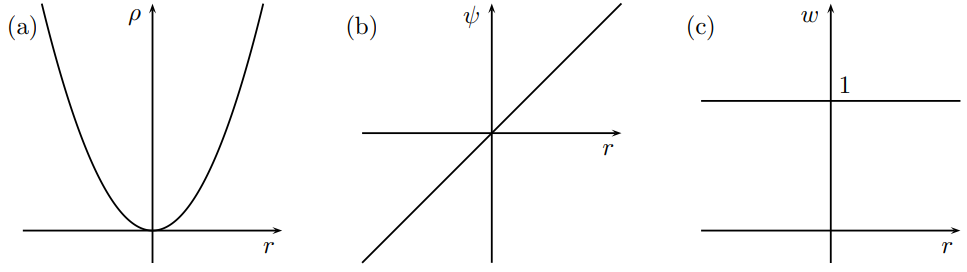
\includegraphics[width=\linewidth]{Pics/10.4.1.png}
  \caption{Loss function $\rho$ of least-squares estimate (a), $\psi$-function (b) and corresponding weight function $w$ (c).}
\end{figure}
\begin{figure}[H]
  \centering
  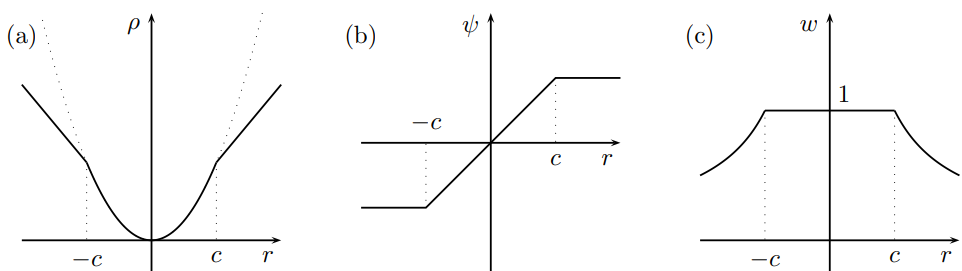
\includegraphics[width=\linewidth]{Pics/10.4.2.png}
  \caption{Loss function $\rho$ (a) of Huber’s $\psi$-function (b) and corresponding weight function $w$ (c).}
\end{figure}
The corresponding weights are then simply
\begin{equation}
  w_i = \frac{\psi (e_i)}{e_i}
\end{equation}
The threshold $c$ in Huber’s $\psi$-function is set to be $c = 1.345$ which is based on theoretical efficiency considerations.\\
The regression M-estimation limits only the influence of large residuals, but is still prone to leverage points and therefore has a break point of zero. To be able to handle bad leverage points we need a redescending $\psi$-function such that observations with large absolute residuals are gradually ignored.\\

\textbf{Modified Robust Regression M-Estimator}\\
\begin{figure}[H]
  \centering
  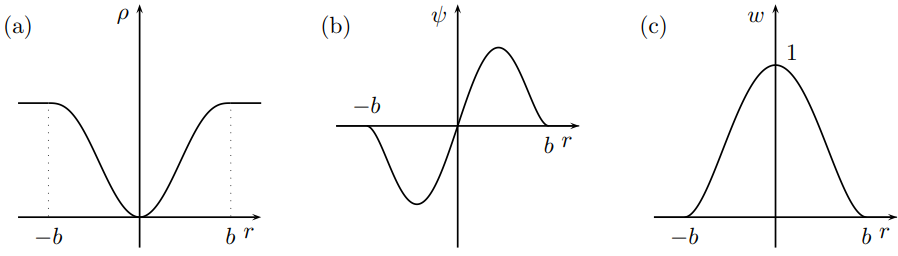
\includegraphics[width=\linewidth]{Pics/10.4.5.png}
  \caption{Loss function $\rho$ (a) of Tukey's bisquare $\psi$-function (b) and corresponding weight function $w$ (c).}
\end{figure}
The threshold $b$ of Tukey’s bisquare is set to be $b = 4.685$ which is based on theoretical efficiency considerations. The regression MM-estimator has a breakdown point of $\frac{1}{2}$ and an efficiency and an asymptotic distribution like the regression M-estimator.

\section{Variable Selection and Modeling}
\noindent\rule[\linienAbstand]{\linewidth}{\linienDickeDick}

In practice, regression is used in many situations. The approach depends on the previous knowledge and subject-specific questions.\\
\begin{itemize}
  \item Ideally, the relationships between the response $y$ and the explanatory variables $x_1, ..., x_m$  is clear in advance. The functional relationships are often based on physical, chemical or other engineering or scientific theory. We call these \textbf{mechanistic models}. In this case we are most often interested in good estimates of the parameters, confidence and prediction intervals.
  \item  In the other case, the study serves to investigate relationships between the response variable x and the explanatory variables. We do not know if and in what form the explanatory variables influence the response. The functional relationships are unknown and so we have to find \textbf{empirical models}.
  \item Sometimes the approach is in between: If we are only interested in the influence of a single explanatory variable, but take into account the effects of other explanatory variables, or if a lot of previous studies and theoretical considerations is known and additional knowledge should be gained.
\end{itemize}

\subsection{Model Selection Methods}
\noindent\rule[\linienAbstand]{\linewidth}{\linienDicke}
We will proceed the approach with model selection methods which are based on statistical measures of goodness of fit.
In the following we will define three statistical measures of model accuracy which also take the model complexity into consideration.
\begin{itemize}
  \item Adjusted R-squared
  \item Akaike information criterion $(AIC)$
  \item Mallow’s $C_p$ statistic is
\end{itemize}
With these model selection criteria, three different variable selection methods can be formulated:

\begin{itemize}
  \item Forward selection
  \begin{enumerate}
    \item In the first step choose the trivial model $y = \beta_0 + \varepsilon$ with an intercept only. Use \texttt{formula = y $\sim$ 1} in R.
    \item In the following steps, the explanatory variable that leads to the largest improvement of the selected model selection criteria is added in the model.
    \item The procedure is stopped as soon as no improvement is possible by adding another explanatory variable.
  \end{enumerate}

  \item Backward elimination
  \begin{enumerate}
    \item In the first step choose the full model
    \begin{equation}
      y = \beta_0 + \beta_1 x_1 + \beta_2 x_2 + \dots + \beta_m x_m + \varepsilon
    \end{equation}
    with all possible explanatory variables. Use \texttt{formula = y $\sim$ .} in R.
    \item In the following steps, the explanatory variable that leads to the largest improvement of the selected model selection criteria is removed from the model.
    \item The procedure is stopped as soon as no improvement is possible by removing another explanatory variable.
  \end{enumerate}

  \item \emph{Both} is a combination of forward selection and backward elimination.
  \begin{enumerate}
    \item In the first step choose any model.
    \item The following steps will examine whether eliminating or adding an explanatory variable improves the selected model selection criteria. The action that leads to  the largest improvement is carried out.
    \item The procedure is stopped as soon as no improvement is possible.
  \end{enumerate}
\end{itemize}


\subsection{Collinearity}
\noindent\rule[\linienAbstand]{\linewidth}{\linienDicke}
Collinearity means that an explanatory variable $x_j$ can almost be represented by the others as a linear combination.
\begin{equation}
  x_k \approx \gamma_0 + \sum^m_{j, j\neq k}\gamma_j x_j
\end{equation}
If this relation is exakt then the least-squares estimator is not uniquely defined and software implementations may have problems.\\

\textbf{Measure for Collinearity}\\
If the equation above is only approximately satisfied we can consider it as a linear multiple regression model. For each explanatory variable $x_k$ define the coefficient of determination $R^2_k$ of the model. The \textbf{variance inflation factor} of variable $x_k$ is then defined by
\begin{equation}
  \textup{VIF}_k = \frac{1}{1-R^2_k}
\end{equation}
It is a good and easy to calculate measure of collinearity. A rule of thumb is that if this measure is greater than 5, there are problems with collinearity.\\
High collinearity leads to large standard errors of the estimated coefficients. It is possible to show, that the standard error of the estimate of the coefficient $\beta_k$ is increased by a factor of
\begin{equation}
  \sqrt{\textup{VIF}_k}
\end{equation}
In an ideal situation with no collinearity we would have $R^2_k = 0$ and therefore $\textup{VIF}_k = 1$ and hence no increase in the standard error of the estimated coefficient $\hat{\beta}_k$.

\subsection{Modelling Strategies}
\noindent\rule[\linienAbstand]{\linewidth}{\linienDicke}
In statistical regression modelling we have dealt with three important elements:
\begin{itemize}
  \item \textbf{Residual analysis}. In the residual analysis, we check as well as possible the assumptions of independence, constant variance, linearity and normal distribution. We also try to identify influential observations. Robust methods are suitable for carrying out this analysis very efficiently.
  \item \textbf{Transformations}. Depending on the situation, it makes sense to transform the response as well as the explanatory variables, to add interactions or to expand the models with factor variables.
  \item \textbf{Variable selection}. Nowadays, it is easy to automatically select explanatory variables. That this is not in any case advisable and has been explained at the beginning of this section.
\end{itemize}

\textbf{Overall Strategy}
\begin{enumerate}
  \item Understand the problem. Are there already approaches for models available?
  \item Collect and process data.
  \begin{itemize}
    \item Clarify the coding of missing values (sometimes coded with -99 or 0). Define the treatment of missing values in the analysis.
    \item Unify the meaning of the number 0 in different variables.
    \item Treat data according to first-aid transformations unless there are valid reasons against it (eg. existing model).
    \item Keep track of the data quality when merging multiple data sets. The overall quality is never higher than the weakest link.
  \end{itemize}
  \item First model fit (preferably with robust methods).
  \item Residual analysis. Does the data help to solve the question? If not, repeat the first,
  second and third step.
  \item Variable selection, treat collinearity if necessary.
  \item Check goodness of fit.
  \begin{itemize}
    \item Residual analysis with selected models.
    \item Match models with first principles.
    \item Validate models with data not used in modelling.
  \end{itemize}
\end{enumerate}

\textbf{Final Remarks}\\
In this introduction, important elements of multiple linear regression analysis have been addressed. Lots of different generalisations exist and go in different directions.
\begin{itemize}
  \item \textbf{Nonlinear regression}. More complicated functions can be fitted.
  \item \textbf{Nonparametric regression}. Less assumptions on the models are made (smoothing).
  \item \textbf{Generalised linear model}. The response variable is allowed to have error distribution models other than the normal distribution (logistic, Poisson and gammaregression).
  \item \textbf{Survival analysis}. Censored data (reliability theory, survival and hazard function).
  \item \textbf{Time series analysis}. The errors can be correlated.
  \item \textbf{Principal component} and \textbf{partial least squares regression}. (Many) more variables than observations are available: large $p$, small $n$ (chemometrics).
\end{itemize}


% Part III
\part{Design of Experiment}
\section{Design of Experiment}
\noindent\rule[\linienAbstand]{\linewidth}{\linienDickeDick}
Many scientific studies are concerned with the understanding of causal relationships. Statistical design of experiment (DoE) refers to the process of planning an experiment so that the data can be evaluated with statistical methods in a convenient way. However, the evaluation as well as the quality of the results essentially depends on the chosen test plan.\\

In this third part we will be interested in the following aspects.
\begin{itemize}
  \item \textbf{Comparison of treatments}. The most common aim in an experiment is to compare several treatments and to choose the best one.
  \item \textbf{Variable screening}. If there are lot of potentially influential factors in a process it is common to try to find the most important factors with a systematic screening experiment.
  \item \textbf{Response surface methodology}. If once the most important factors of a process are determined the optimal setting of these factors is often searched.
\end{itemize}

\subsection{Terminology and Concepts}
\noindent\rule[\linienAbstand]{\linewidth}{\linienDicke}
In general the response variable depends on many explanatory variables which can be separated in two groups.
\begin{itemize}
  \item \textbf{Primary variables} are directly connected with the study.
  \item \textbf{Secondary variables} are also controllable with a reasonable effort.
\end{itemize}
\textbf{Basic idea of an experiment:} Primary and secondary variables can be varied in a prescribed controlled manner.\\

\textbf{Random error:} Sum of all unknown influences.\\

\textbf{Balanced design:} Design with factor variables\\

\textbf{Orthigonal design:} Design with continuous variables.\\

\textbf{Block designs:} Record additional variables, i.e. batches, production lot or origin of product.
\begin{itemize}
  \item Precision can be increased (if variable is significant).
  \item Interpretability of the results can be simplified.
\end{itemize}

\textbf{Randomisation:} Perform experiments in random order
\begin{itemize}
  \item Chronological order as independent as possible from all recorded and unrecorded variables.
  \item Prevent influences due to the system of the experimental conditions.
  \item Avoid learning effects or aging of a device.
\end{itemize}

\textbf{Replicates:} Multiple measurements with same experimental conditions.
\begin{itemize}
  \item Improved accuracy of the statements.
  \item Estimate of the variation of the random errors available.
  \item Existence of interactions in analysis of variance can be tested.
  \item Replicates are not allowed to be measured consecutively, otherwise they are not independent.
  \item Randomise replicates despite the increased experimental effort.
\end{itemize}

\subsection{Experimental Design}
\noindent\rule[\linienAbstand]{\linewidth}{\linienDicke}
\textbf{Design of Experiment - Basic Principles}
\begin{itemize}
  \item The main question defines the response variable and the primary explanatory variables   and their relevant value range.
  \item Record as many variables which might have an influence on the response as possible.   These secondary variables should, if possible, be kept constant or used for blocking. If   this is not possible, they should still be considered in the model.
  \item All explanatory variables should be orthogonal and the factors balanced.
  \item The assignment of experimental conditions to study units should be randomised.
  \item Independent replicates allow additional model validation
\end{itemize}

\textbf{Experimental design:} : List of experimental conditions that determine how each factor is to be varied and at which levels.\\

\textbf{Completely randomised design:}
\begin{itemize}
  \item One multi-level primary factor variable.
  \item One or more (but always the same number) measurements are made per level.
  \item The design is processed in random order to avoid systematic effects.
\end{itemize}

\textbf{Complete block design:}
\begin{itemize}
  \item A secondary factor influences the target variable in addition to the primary factor.
  \item Every level of the primary factor (eg. treatment) is used at least once in each block.
\end{itemize}

\textbf{Complete factorial design:}
\begin{itemize}
  \item Examine $k$ factors with $L$ levels each.
  \item Design with $L^k$ measurements is needed.
  \item Often too many measurements.
\end{itemize}

\textbf{$2^k$ factorial designs:}
\begin{itemize}
  \item In screening experiments, many factors are investigated for their influence on the response variable.
  \item Examine only 2 levels (high and low) per factor.
\end{itemize}

\textbf{$2^k$ fractional factorial designs:}
\begin{itemize}
  \item To save even more resources.
  \item Only a balanced part of the complete $2^k$ design is realised.
\end{itemize}

\subsection{Planning and Conducting a Study}
\noindent\rule[\linienAbstand]{\linewidth}{\linienDicke}
\begin{enumerate}
  \item \textbf{Scientific question:} Avoid situations without precise questions and hypotheses.
  \item \textbf{Response and explanatory variables:} Find all influential factors, eg. with a cause-and-effect diagram.
  \item \textbf{Preliminary experiments:} Experience with the topic and the measurement equipment is important.
  \item \textbf{Planning:} It is worth going through the question, eg. with simulated data. The evaluation of the data in relation to the main questions is clear.
  \item \textbf{Sample size:} The magnitude of the random fluctuations and the size of the expected effects has to be known. Often, the question must be downsized.
  \item \textbf{Data:} It is important to keep a journal that documents the process of data acquisition and highlights any peculiarities and unforeseen circumstances that may later explain unexpected data discrepancies.
  \item \textbf{Data cleanup:} Checking the plausibility of the data and visualising it saves a lot of effort.
  \item \textbf{Evaluation, interpretation:} The methodology for evaluating the data in relation to the main question is clear.
  \item \textbf{Report, presentation:} For whom is the report mainly intended?
  \item \textbf{Completion:} It is worthwhile to collect and discuss the experiences made with all participants.
\end{enumerate}

\section{Factorial Designs and Analysis of Variance}
\noindent\rule[\linienAbstand]{\linewidth}{\linienDickeDick}
In regression and analysis of variance we are interested in situations with only one response variable which is directly measurable or observable. In general this response variable is influenced by several explanatory variables or factors. The knowledge of the explanatory variables and factors is essential to be able to interpret the response correctly.

\subsection{One Factor Analysis of Variance}
\noindent\rule[\linienAbstand]{\linewidth}{\linienDicke}
With the one factor analysis of variance we want to check whether a factor (for example the hardwood concentration in paper) has a significant effect.\\
We check this by asking if there is a difference between one group and another group. The corresponding hypothesis are:
\begin{equation}
  \begin{split}
    H_0 &= \mu_1 = \mu_2 = \dots = \mu_g \; \text{(i.e. all groups obey the same model)}\\
    H_1 &= \mu_i \neq \mu_j \;\text{j for at least one pair}\; i, j \;\text{with}\; i \neq j.
  \end{split}
\end{equation}
We describe the situation with a linear model. We want to compare $g$ groups with $m$ measurements each. The model where individual observations within the $i$th group scatter randomly around a common value $\mu_i$ is described by
\begin{equation}
  y_{ij} = \mu_i + \varepsilon_{ij} \;\text{with}\; i \in \{1, 2, ..., g\} \;\text{and}\; j \in \{1, 2, ...,m\}
\end{equation}
Notice that the model can also be written as
\begin{equation}
  y_{ij} = \mu + \tau_i + \varepsilon_{ij} \;\text{with}\; i \in \{1, 2, ..., g\} \;\text{and}\; j \in \{1, 2, ...,m\}
\end{equation}
with corresponding hypothesis
\begin{equation}
  \begin{split}
    H_0 &: \; \tau_1 = \tau_2 = \dots = \tau_g = 0\\
    H_1 &: \; \tau_i \neq 0 \;\text{for at least one i}.
  \end{split}
\end{equation}
The parameter $\mu$ is common to all treatments called the overall mean, $\tau_i$ is a parameter associated with the $i$th treatment called the $i$th treatment effect.\\

We are looking for a test statistic that takes extreme values if the means $(\bar{y}. \;\text{with the "."})$ of the $g$ groups differ. If the variance
of the group means $S_b^2$ compared to the variance of the observations within the groups $S_w^2$ is large, then we reject the null hypothesis. Therefore the test statistics for the analysis of variance test (ANOVA) is
\begin{equation}
  \begin{split}
    F &= \frac{\text{variance between groups}}{\text{variance within groups}} = \frac{S_b^2}{S_w^2}\\
    &= \frac{\frac{1}{g-1} \sum_{i=1}^g m\left(\bar{y}_{i.} - \bar{y}_{i..}\right)^2}{\frac{1}{n-g} \sum_{i=1}^g \sum_{j=1}^m \left(\bar{y}_{ij} - \bar{y}_{i.}\right)^2}
  \end{split}
\end{equation}
where $\bar{y}..$ is the estimated overall mean.\\
The terms leading to the test statistic $F$ are summarised in the following analysis of variance table.
\begin{table}[H]
  \centering
  \footnotesize
  \begin{tabular}{ m{1.5cm} | m{1cm} ll}
      Source of Variation  & Sum of Squares & Degrees of Freedom & Mean Squares \\ \hline
      Tratments (groups)  & $\textup{SS}_G$ & $\textup{df}_G = g-1$ & $\textup{MS}_G = \frac{\textup{SS}_G}{\textup{df}_G}$\\
      Error (residuals)   & $\textup{SS}_E$ & $\textup{df}_E = n-g$ & $\textup{MS}_E = \frac{\textup{SS}_E}{\textup{df}_E}$\\ \hline
      Total               & $\textup{SS}_T$ & $\textup{df}_T = n-1$ &\\
  \end{tabular}
\end{table}

The sums of squares are defined by
\begin{equation*}
  \begin{split}
    \textup{SS}_G &= \sum_{i=1}^g m\left(\bar{y}_{i.} - \bar{y}_{..}\right)^2\\
    \textup{SS}_E &= \sum_{i=1}^g \sum_{j=1}^m \left(y_{ij} - \bar{y}_{i.}\right)^2\\
    \textup{SS}_T &= \sum_{i=1}^g \sum_{j=1}^m \left(y_{ij} - \bar{y}_{..}\right)^2
  \end{split}
\end{equation*}
It is possible to show that
\begin{equation}
  SS_T = SS_G + SS_E
\end{equation}

The test statistic of the analysis of variance test can also be written as
\begin{equation}
  F = \frac{\textup{MS}_G}{\textup{MS}_E}
\end{equation}
Under the null hypothesis the $F$-statistic follows an $F$-distribution with $(\textup{df}_G, \textup{df}_E) = (g - 1, n - g)$ degrees of freedom. Critical values of the $F$-distribution can be found in tables.

\subsection{Two Factor Analysis of Variance}
\noindent\rule[\linienAbstand]{\linewidth}{\linienDicke}
The one factor analysis of variance is the generalisation of the comparison of two independent samples. We can further generalise to the analysis of variance with several factors.\\
Suppose that we have two factors $A$ and $B$ with $a$ and $b$ levels. A model which is capable to separate real effects from random fluctuations can be built as follows
\begin{equation}
  y_{ij} = \mu_{ij} + \varepsilon_{ij} \;\text{with}\; i \in \{1, 2, ..., a\} \;\text{and}\; j \in \{1, 2, ...,b\}
\end{equation}
In this model every observation $y_{ij}$ has a random deviation $\varepsilon_{ij}$ from an ideal value $\mu_{ij}$ which depends on the method $i$ and the batch $j$. More precisely the ideal value
\begin{equation}
  \mu_{ij} = \mu + \alpha_i + \beta_j
\end{equation}
is based on an overall value $\mu$, an effect $\alpha_i$ which describes the factor $A$ and an effect $\beta_j$ which describes the factor $B$.\\
To be able to estimate the parameters uniquely we need to assume two constraints
\begin{equation}
  \sum_{i=1}^{a} \alpha_i = 0 \;\;\; \text{and} \;\;\; \sum_{j=1}^b \beta_j = 0
\end{equation}

The parameters $\mu, \alpha_1, \alpha_2, . . . , \alpha_a$ and $\beta_1, \beta_2, . . . , \beta_b$ can be estimated from the model
\begin{equation}
  y_{ij} = \mu + \alpha_i + \beta_j + \varepsilon_{ij} \;\text{with}\; i \in \{1, 2, ..., a\} \;\text{and}\; j \in \{1, 2, ...,b\}
\end{equation}
For every level $i$ and $j$ we obtain
\begin{equation}
  \begin{split}
    \bar{y}_{i.} =& \; \mu + \alpha_i\\
    \bar{y}_{.j} =& \; \mu + \beta_j\\
    \bar{y}_{..} =& \; \mu
      \end{split}
\end{equation}

All together we obtain the estimates
\begin{equation}
  \begin{split}
    \hat{\mu} &= \bar{y}_{..}\\
    \hat{\alpha}_i &= \bar{y}_{i.} - \bar{y}_{..} \;\text{for all}\; i \in \{1, 2, ..., a\}\\
    \hat{\beta}_i &= \bar{y}_{.j} - \bar{y}_{..}  \;\text{for all}\; j \in \{1, 2, ..., b\}\\
  \end{split}
\end{equation}

As a basis for statistical tests we set up a variance analysis table for two factors which is an extension
of the one factor analysis of variance table.
\begin{table}[H]
  \footnotesize
  \centering
  \begin{tabular}{ m{1.5cm} | m{1cm} l m{0.8cm} m{1.2cm}}
      Source of Variation  & Sum of Squares &  Degrees of Freedom & Mean Squares & Test Statistic \\ \hline
      Factor A   & $\textup{SS}_A$ & $\textup{df}_A = a-1$     & $\textup{MS}_A$ & $\textup{MS}_A / {MS}_E$\\
      Factor B   & $\textup{SS}_B$ & $\textup{df}_B = b-1$     & $\textup{MS}_B$ & $\textup{MS}_B / {MS}_E$\\
      Error      & $\textup{SS}_E$ & $\textup{df}_E = n-a-b+1$ & $\textup{MS}_E$ & \\ \hline
      Total      & $\textup{SS}_T$ & $\textup{df}_T = n-1$     &                 &\\
  \end{tabular}
\end{table}
The sums of squares are defined by
\begin{equation}
  \begin{split}
    \textup{SS}_A &= \sum_{i=1}^a \sum_{j=1}^b \hat{\alpha}_i^2 = b \sum_{i=1}^a \hat{\alpha}_i^2\\
    \textup{SS}_B &= \sum_{i=1}^a \sum_{j=1}^b \hat{\beta}_j^2 = b \sum_{j=1}^b \hat{\beta}_j^2\\
    \textup{SS}_E &= \sum_{i=1}^a \sum_{j=1}^b \hat{e}_{ij}^2\\
    \textup{SS}_T &= \sum_{i=1}^a \sum_{j=1}^b \left(y_{ij} - \bar{y}_{..}\right)^2
  \end{split}
\end{equation}

We test the alternative hypothesis
\begin{equation}
  \begin{split}
    H_0 &: \alpha_1 = \alpha_2 = \dots = \alpha_a = 0\;\\
    H_1 &: \alpha_i \neq 0 \;\text{for at least one i}.
  \end{split}
\end{equation}
i.e. all effects of the factor $A$ are zero, with the test statistic
\begin{equation}
  F_A = \frac{\textup{MS}_A}{\textup{MS}_E} = \frac{\frac{\textup{SS}_A}{\textup{df}_A}}{\frac{\textup{SS}_E}{\textup{df}_E}}
\end{equation}
Under the null hypothesis the statistic follows an $F$-distribution with
\begin{equation}
  \left(\textup{df}_A, \textup{df}_E\right) = (a - 1, n - a - b + 1) = (a - 1,(a - 1)(b - 1))
\end{equation}
degrees of freedom. Critical values of the $F$-distribution can be found in tables. Analogously, we can test the factor $B$.

\subsection{Two Factor Analysis of Variance with Interaction}
\noindent\rule[\linienAbstand]{\linewidth}{\linienDicke}
So far, it has been assumed that for each combination $(i, j)$ of one level of factor $A$ with one level of factor $B$, only one observation $y_{ij}$ is recorded. In the simplest model with $c$ observations per combination $(i, j)$, one more index $k$ has to be added to the previous model.
\begin{equation}
  \mu_{ijk} = \mu + \alpha_i + \beta_j + \varepsilon_{ijk}
\end{equation}
with $i \in \{1, 2, . . . , a\}, j \in \{1, 2, . . . , b\}$ and $k \in \{1, 2, . . . , c\}$. The observations on the same combination $(i, j)$ are called \textbf{replicates}.\\

If the polygonal lines in the interaction plot are not almost parallel, then the additive model has to be modified too. The model with two factors and an \textbf{interaction} is
\begin{equation}
  \mu_{ijk} = \mu + \alpha_i + \beta_j + \gamma_{ij} + \varepsilon_{ijk}
\end{equation}
with $i \in \{1, 2, . . . , a\}, j \in \{1, 2, . . . , b\}$ and $k \in \{1, 2, . . . , c\}$. To be able to properly estimate the coefficients we have to add further constraints on the interaction term $\gamma_{ij}$
\begin{equation}
  \sum_{i=1}^{a} \gamma_{ij} = 0 \;\;\; \text{and} \;\;\; \sum_{j=1}^b \gamma_{ij} = 0
\end{equation}

It is very important to know that the parameter estimate of the model with interaction, needs more than one observation per combination $(i, j)$. The estimates for the parameters can be found analogously as in the chapter above, for the model with two factors. We obtain the estimates
\begin{equation}
  \begin{split}
    \hat{\mu}         &= \bar{y}_{...}\\
    \hat{\alpha}_i    &= \bar{y}_{i..} - \bar{y}_{...} \;\text{for all}\; i \in \{1, 2, ..., a\}\\
    \hat{\beta}_i     &= \bar{y}_{.j.} - \bar{y}_{...}  \;\text{for all}\; j \in \{1, 2, ..., b\}\\
    \hat{\gamma}_{ij} &= \bar{y}_{ij.} - \bar{y}_{i..} - \bar{y}_{.j.} + \bar{y}_{...}  \;\text{for all}\; i \in \{1, 2, ..., a\},\;j \in \{1, 2, ..., b\}\\
  \end{split}
\end{equation}
As a basis for statistical tests we set up a variance analysis table for two factors with an interaction:
\begin{table}[H]
  \footnotesize
  \centering
  \begin{tabular}{ m{1.6cm} | m{0.9cm} l m{0.8cm} m{1.2cm}}
      Source of Variation  & Sum of Squares &  Degrees of Freedom & Mean Squares & Test Statistic \\ \hline
      Factor A      & $\textup{SS}_A$ & $\textup{df}_A = a-1$        & $\textup{MS}_A$ & $\textup{MS}_A / {MS}_E$\\
      Factor B      & $\textup{SS}_B$ & $\textup{df}_B = b-1$        & $\textup{MS}_B$ & $\textup{MS}_B / {MS}_E$\\
      Interaction I & $\textup{SS}_I$ & $\textup{df}_I = (a-1)(b-1)$ & $\textup{MS}_I$ & $\textup{MS}_I / {MS}_E$\\
      Error         & $\textup{SS}_E$ & $\textup{df}_E = ab(c-1)$    & $\textup{MS}_E$ & \\ \hline
      Total         & $\textup{SS}_T$ & $\textup{df}_T = n-1$        &                 &\\
  \end{tabular}
\end{table}
The sums of squares are defined by
\begin{equation}
  \begin{split}
    \textup{SS}_A &= bc \sum_{i=1}^a \hat{\alpha}_i^2\\
    \textup{SS}_B &= ac \sum_{i=1}^b \hat{\beta}_j^2\\
    \textup{SS}_E &= \sum_{i=1}^a \sum_{j=1}^b \sum_{k=1}^c \hat{e}_{ijk}^2\\
    \textup{SS}_T &= \sum_{i=1}^a \sum_{j=1}^b \sum_{k=1}^c \left(y_{ijk} - \bar{y}_{...}\right)^2
  \end{split}
\end{equation}
and
\begin{equation}
  \textup{SS}_I = \textup{SS}_T - \textup{SS}_A - \textup{SS}_B - \textup{SS}_E
\end{equation}
We test the alternative hypothesis
\begin{equation}
  \begin{split}
    H_0 &: \gamma_{11} = \gamma_{12} = \gamma_{13} \dots = \gamma_{ab} = 0\;\\
    H_1 &: \gamma_{ij} \neq 0 \;\text{for at least one combinationi}\;(i,j).
  \end{split}
\end{equation}
i.e. all effects of the interaction $I$ are zero, with the test statistic
\begin{equation}
  F_I = \frac{\textup{MS}_I}{\textup{MS}_E} = \frac{\frac{\textup{SS}_I}{\textup{df}_I}}{\frac{\textup{SS}_E}{\textup{df}_E}}
\end{equation}
Under the null hypothesis the statistic follows an $F$-distribution with
\begin{equation}
  (\textup{df}_I , \textup{df}_E) = (ab(c - 1),(a - 1)(b - 1))
\end{equation}
degrees of freedom.\\
Since a block cannot interact with the treatment, no interactions with block designs are allowed.\\

\subsection{Residual Analysis}
\noindent\rule[\linienAbstand]{\linewidth}{\linienDicke}
Analysis of variance and regression are very similar. It is also an essential step in analysis of variance to check the model assumptions with the help of residual analysis. Almost all the tools previously mentioned can also be used in analysis of variance: Tukey-Anscombe plot, scale-location plot, q-q plot, residuals versus explanatory variables and residuals versus time.\\
In analysis of variance the residuals versus leverage is not useful, since all explanatory variables
have the same leverage.

\section{Screening Experiments}
\noindent\rule[\linienAbstand]{\linewidth}{\linienDickeDick}

\subsection{2k Factorial Designs}
\noindent\rule[\linienAbstand]{\linewidth}{\linienDicke}
\subsection{2k Fractional Factorial Designs}
\noindent\rule[\linienAbstand]{\linewidth}{\linienDicke}

\section{Response Surface Methodology}
\noindent\rule[\linienAbstand]{\linewidth}{\linienDickeDick}

Response surface methodology (RSM) is a statistical technique which is used to model and analyse processes and data in applications in which a response of interest is influenced by several explanatory variables and the aim is to optimise this response.\\
To find the optimum settings of the explanatory variables, it may be useful to proceed in three steps:
\begin{enumerate}
  \item A $2^k$ factorial design (possibly fractional) is used to detect the important influencing factors.
  \item For the most important influencing factors, the main effects are estimated in order to determine the direction of the steepest ascent.
  \item Now we can hope to find the global optimum in the determined direction with a suitabledesign and additional experiments.
\end{enumerate}
This kind of procedure is a response surface exploration which is based on a sequence of experimental design.


\subsection{Response Surface}
\noindent\rule[\linienAbstand]{\linewidth}{\linienDicke}
In the search for relevant influencing factors, we assumed two (or more) levels per factor and used the analysis of variance to estimate and test main effects (and interactions). The model for two factors $A$ and $B$ with two levels each and without interaction is
\begin{equation}
  y_{ij} = \mu_{ij} + \varepsilon_{ij} = \mu + \alpha + \beta_j + \varepsilon_{ij}
\end{equation}

If both explanatory variables $x_1$ and $x_2$ are continuous then the model is
\begin{equation}
  y = f(x_1, x_2) + \varepsilon
\end{equation}
where $\varepsilon$ represents the noise or error observed in the response $y$.
If we denote the expected response by $E(y) = f(x_1, x_2) = \eta$, then the surface represented by
\begin{equation}
  \eta = f(x_1, x_2) + \varepsilon
\end{equation}
is called a response surface.\\

We start with a so-called \textbf{first-order design}, a $2^k$ design with additional measurements in the center of the test conditions.\\
If the response is well modeled by a linear function of the $k$ explanatory variables, the approximating function is the \textbf{first-order model}
\begin{equation}
  y = \beta_0 + \beta_1 x_1 + \beta_2 x_2 + \dots + \beta_k x_k + \varepsilon
\end{equation}

\textbf{Example}\\
A first-order test design and the results of the measurement are reported in the following table.
\begin{table}[H]
  \centering
  \scriptsize
    \begin{tabular}{c|cc|cc|c}
      Run & \multicolumn{2}{c}{Variables in}   & \multicolumn{2}{c}{Variables in} & Yield \\
          & \multicolumn{2}{c}{original units} & \multicolumn{2}{c}{coded untis}  &       \\
          & $T$ [°C] & $t$ [min]               & $\texttt{Temp}$ & $\texttt{Time}$ & y [g]\\ \hline
      1 & 120 & 50 & $-1$ & $-1$ & 52.3 \\
      2 & 160 & 50 & $+1$ & $-1$ & 62.2 \\
      3 & 120 & 70 & $-1$ & $+1$ & 60.1 \\
      4 & 160 & 70 & $+1$ & $+1$ & 70.7 \\ \hline
      5 & 140 & 60 &   0  &   0  & 63.5 \\
      6 & 140 & 60 &   0  &   0  & 63.6
    \end{tabular}
\end{table}
The design is given in coded form and in original units.\\
Now we fit this model to the data of the $2^2$ design with two additional measurements (runs 5 and 6) in the centre of the test conditions.\\
The gradient of the response function
\begin{equation}
  f(\texttt{Temp, Time}) = \beta_0 + \beta_1 \cdot \texttt{Temp} + \beta_2 \cdot \texttt{Time}
\end{equation}
is
\begin{equation}
  \text{grad}\left(f(\texttt{Temp, Time})\right) =
  \begin{pmatrix} \beta_1 \\ \beta_2 \end{pmatrix} =
  \begin{pmatrix} 5.125 \\ 4.075 \end{pmatrix}
\end{equation}
The estimated gradient points into the direction of the largest change in the coded $\texttt{Temp-Time}$-domain. Notice that this direction leads us to a maximal increase of the response.

\begin{figure}[H]
  \centering
  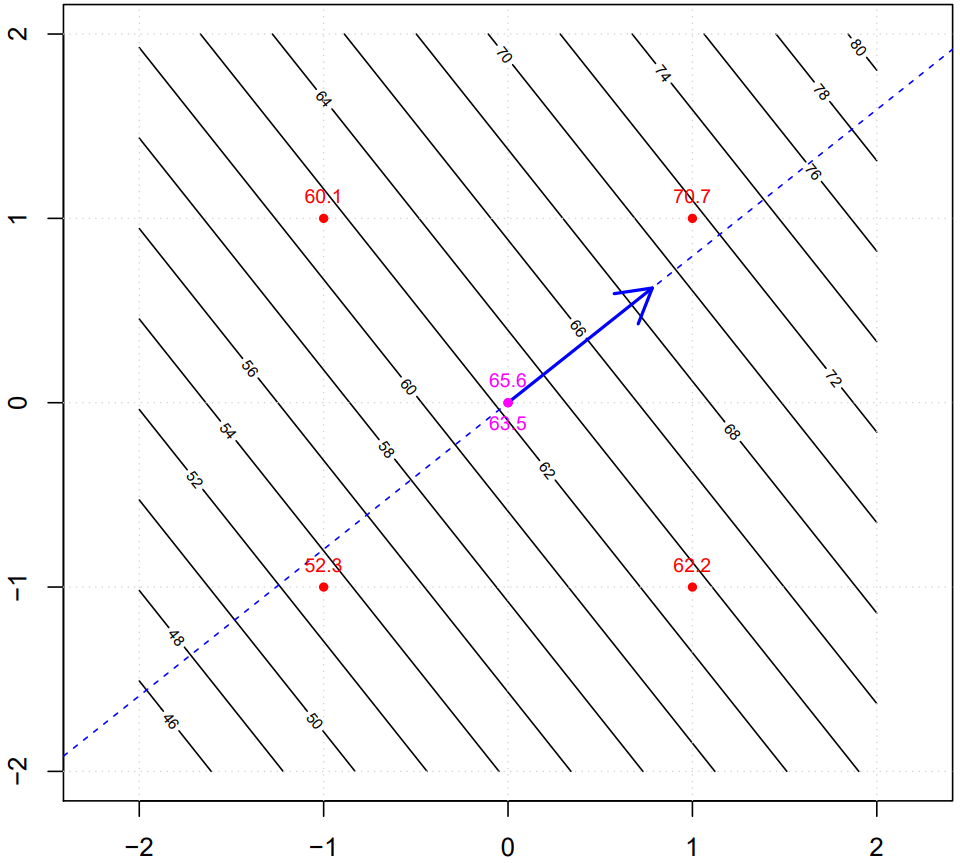
\includegraphics[width=.6\linewidth]{Pics/15.1.2.png}
\end{figure}

There are two reasons why we extended the $2^2$ design with two additional measurements in the centre of the test conditions.
\begin{itemize}
  \item If several measurements for that point are made, then the measurement error can be determined without assuming that the first-order linear model approximates the true response sufficiently well.
  \item It is possible to detect deviations (curvature) from the first-order linear model. If no curvature is present and if the plane is a sufficient approximation of the response within the experimental domain, then the mean of the central observations $\bar{y}_c$ and the mean of all the other observations in the $2^k$ factorial design $\bar{y}_f$ are almost the same. If, on the other hand, this difference is significantly different from zero then this is an indication that a model with curvature is more appropriate.\\
\end{itemize}

The corresponding hypothesis to test the presence of curvature in a $2^k$ design are
\begin{equation}
  \begin{split}
    H_0 &: \;\text{no curvature in the data},\\
    H_1 &: \;\text{curvature in the data}.
  \end{split}
\end{equation}

The test statistic for the curvature in a $2^k$ factorial design is
\begin{equation}
  t_{\text{curve}} = \frac{\bar{y}_c -\bar{y}_f}{\sqrt{s_c^2 \left(\frac{1}{n_c} + \frac{1}{2^k}\right)}}
\end{equation}
Where $s_c^2$ is the empirical variance.
Under the null hypothesis the test statistic $t_{curv}$ follows a $t$-distribution with $n_c - 1$ degrees of freedom.\\

If the first-order linear model is fits the data well then we can search an optimum along the straight line through the centre of the design and along the estimated gradient.

\subsection{Second-Order Response Surface with Interactions}
\noindent\rule[\linienAbstand]{\linewidth}{\linienDicke}
There are two reasons to use a second-order polynomial:\\
\begin{itemize}
  \item If we are close to the optimum and the estimated response plane is almost horizontal, i.e. the estimated coefficients are almost zero.\\
  \item If there is curvature in the system, then a polynomial of higher degree must be used, such as the second-order model
\end{itemize}
\begin{equation}
  y = \beta_0 + \sum_{i=1}^k \beta_i x_i + \sum_{i=1}^k \beta_{ii} x_i^2 + \sum_{i<j} \beta_{ij} x_i x_j + \varepsilon
\end{equation}
In the case of two explanatory variables the model simplifies to
\begin{equation}
  y = \beta_0 + \beta_1 x_1 + \beta_2 x_2 + \beta_{11} x_{1}^2 + \beta_{22}x_{2}^2 + \beta_{12} x_1 x_2 + \varepsilon
\end{equation}

The $2^k$ design is not enough to estimate the parameters in the second-order model. To keep the effort within limits, so-called \emph{rotatable central composite design} or \emph{second-order central composite design} are used. This design can be obtained from a $2^k$ design by adding more experimental conditions.\\
For the case of two explanatory variables all experimental conditions in coded variables (except the centre) are equidistant from the center $(0, 0)$. Each factor is measured at five levels. $(\pm 1, \pm \sqrt{2}, 0)$\\

\textbf{Example (continuation)}\\
The second-order test plan and the results of the measurements are reported in the following table.
\begin{table}[H]
  \centering
  \scriptsize
    \begin{tabular}{c|cc|cc|c}
      Run & \multicolumn{2}{c}{Variables in}   & \multicolumn{2}{c}{Variables in} & Yield \\
          & \multicolumn{2}{c}{original units} & \multicolumn{2}{c}{coded untis}  &       \\
          & $T$ [°C] & $t$ [min]               & $\texttt{Temp}$ & $\texttt{Time}$ & y [g]\\ \hline
      12 & 195 & 80  & $-1$        & $-1$        & 78.7 \\
      13 & 235 & 80  & $+1$        & $-1$        & 76.2 \\
      14 & 195 & 100 & $-1$        & $+1$        & 72.6 \\
      15 & 235 & 100 & $+1$        & $+1$        & 75.5 \\
      16 & 187 & 90  & $-\sqrt{2}$ & 0           & 74.5 \\
      17 & 243 & 90  & $ \sqrt{2}$ & 0           & 76.2 \\
      18 & 215 & 76  & 0           & $-\sqrt{2}$ & 77.8 \\
      19 & 215 & 104 & 0           & $ \sqrt{2}$ & 72.2 \\
      20 & 215 & 90  & 0           & 0           & 80.7
    \end{tabular}
\end{table}
The second-order linear model in original variables is
\begin{equation}
  y = \beta_0 + \beta_1 T + \beta_2 t + \beta_{11} T^2 + \beta_{22}t^2 + \beta_{12}T\cdot t + \varepsilon
\end{equation}
Now we fit this model with the interaction term to the data in original units of the rotatable central composite design and get the estimated second-order response function.

\begin{figure}[H]
  \centering
  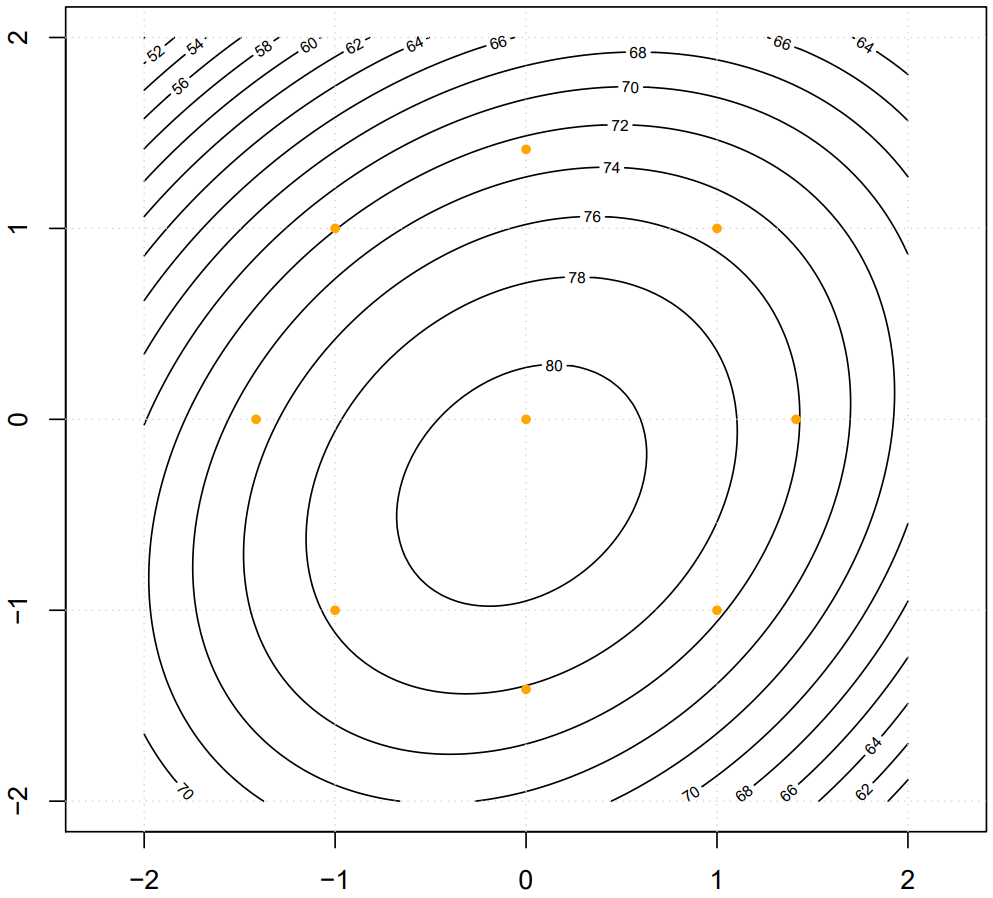
\includegraphics[width=.6\linewidth]{Pics/15.2.1.png}
\end{figure}

A second-order response surface can describe different types of surfaces depending on its parameters.
\begin{itemize}
  \item The surfaces with maximum (or minimum) hardly require any explanation: leaving the optimum in any direction decreases (or increases) the yield $y$.
  \item In the saddle, the yield y may increase or decrease depending on the direction in which the experimental conditions are moving. A fitted saddle is useless to find an optimum.
\end{itemize}

The optimum of the response function can be calculated analytically. The stationary point can be found by setting all $k$ partial derivatives equal to zero.
In the case of two explanatory variables we obtain
\begin{equation}
  \begin{split}
    \frac{\partial}{\partial x_1}f(x_1, x_2) &= \beta_1 + 2\beta_{11} x_1 +  \beta_{12} x_2 = 0 \\
    \frac{\partial}{\partial x_2}f(x_1, x_2) &= \beta_2 +  \beta_{12} x_1 + 2\beta_{22} x_2 = 0
  \end{split}
\end{equation}
and the estimated stationary point is
\begin{equation}
  \hat{x}_1 = \frac{\hat{\beta}_{12} \hat{\beta}_{2} - 2\hat{\beta}_{22} \hat{\beta}_{1}}{4\hat{\beta}_{11} \hat{\beta}_{22} - \hat{\beta}_{12}^2}
  \;\;\;\;\text{and}\;\;\;\;
  \hat{x}_2 = \frac{\hat{\beta}_{12} \hat{\beta}_{1} - 2\hat{\beta}_{11} \hat{\beta}_{2}}{4\hat{\beta}_{11} \hat{\beta}_{22} - \hat{\beta}_{12}^2}
\end{equation}
If the estimated determinant of the Hessian matrix is
\begin{equation}
  4\hat{\beta}_{11} \hat{\beta}_{22} - \hat{\beta}_{12}^2 > 0
\end{equation}
then we have a maximum (or a minimum) otherwise a useless saddle point.\\

\textbf{Summary Response Surface Methodology}\\
\begin{enumerate}
  \item  If the actual settings are far away from the optimum then use a first-order response surface on a $2^k$ fractional factorial design to obtain an overview of the situation.
  \item  Use the method of steepest ascent to obtain further measurements along the gradient till the response gets smaller (larger) again.
  \item  Repeat Step 1 and 2, if necessary, in a vicinity of the optimum found in Step 2.
  \item  Use a rotatable central composite design in the vicinity of the optimum found in Step 3. Estimate the second-order response surface. Find analytically an estimate of the stationary point.
\end{enumerate}

\textbf{All experiments in one plot}\\
\begin{figure}[H]
  \centering
  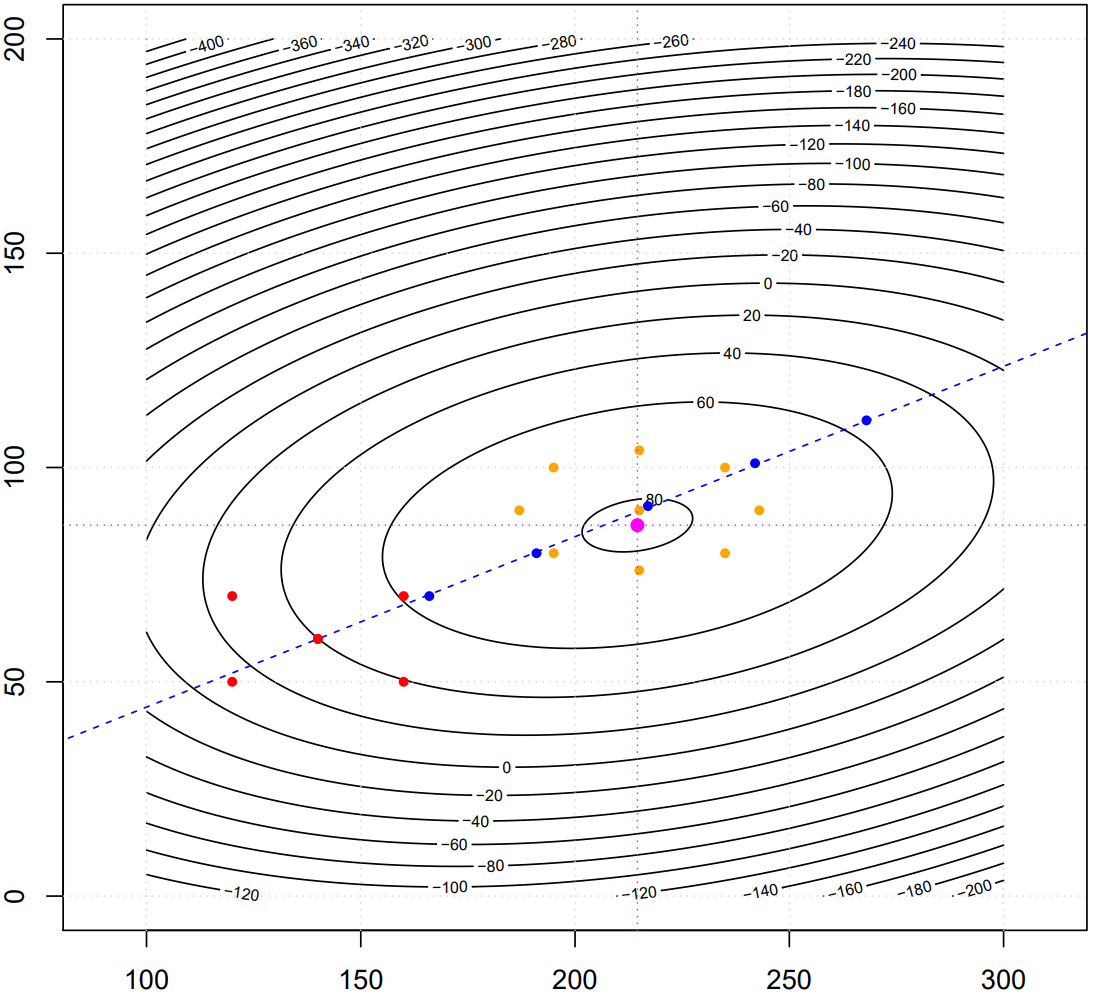
\includegraphics[width=.6\linewidth]{Pics/15.2.3.png}
\end{figure}
Contour plot in original units of the estimated second-order response surface with measurements of the three experiments: Experiment 1 is a $2^2$ factorial design with additional doubled measurement in the centre (red), experiment 2 is an optimisation along the gradient (blue) and experiment 3 is a rotatable central composite design (orange). Optimal settings (magenta).


\part{R}
% \section{R}
% \noindent\rule[\linienAbstand]{\linewidth}{\linienDickeDick}

\section{Basics}
\noindent\rule[\linienAbstand]{\linewidth}{\linienDicke}
\textbf{Normal Distribution Function \texttt{pnorm}}\\
Probability of $X$ being less than 8.10 with $\texttt{mean = 8.00}$ and $\texttt{sd = 0.05}$
\begin{equation*}
  \begin{split}
    P(X \leq 8.10) &= \texttt{pnorm(q=8.10, mean=8.00, sd=0.05)}\\
    &= 0.97725
  \end{split}
\end{equation*}

\textbf{Quantile Function \texttt{qnorm}}\\
Value of $x$ for which $P(X \leq x) = 0.97725$.
\begin{equation*}
  \texttt{qnorm(p=0.97725, mean=8.00, sd=0.05)} = 8.10
\end{equation*}

\section{Utility function for finding sampling plans}
\noindent\rule[\linienAbstand]{\linewidth}{\linienDicke}
\textbf{Description}\\
Find the sampling plan with smallest sample size (single sample only) such that specified Producer Risk Point (PRP) and Consumer Risk Point (CRP) are both met.

\textbf{Arguments}\\
\begin{table}[H]
  \scriptsize
  \begin{tabularx}{\linewidth}{lX}
    \texttt{PRP} &
    The Producer Risk Point in the form of a two element numeric vector of the form \texttt{c(pd, pa)}. The first element, \texttt{pd}, specifies the quality level at which to evaluate the plan. The second element, \texttt{pa}, indicates the minimum probability of acceptance to be achieved by the plan.\\
    \texttt{CRP} &
    The Consumer Risk Point in the form of a two element numeric vector of the form \texttt{c(pd, pa)}. The first element, \texttt{pd}, specifies the quality level at which to evaluate the plan. The second element, \texttt{pa}, indicates the maximum probability of acceptance to be achieved by the plan.\\
    \texttt{type} &
    The distribution which the sampling plan is based on. Possible values are \texttt{binomial, hypergeom, poisson and normal}.\\
    \texttt{N} &
    The size of the population from which samples are drawn. Only applicable for \texttt{type="hypergeom"}.\\
    \texttt{s.type} &
    The type of the standard deviation. A value of known results in a sampling plan based on the population standard deviation, while a value of \texttt{unknown} results in the use of the sample standard deviation.
  \end{tabularx}
\end{table}

\textbf{Usage}\\
\texttt{find.plan(PRP, CRP, type="binomial")}\\
\texttt{find.plan(PRP, CRP, type="hypergeom", N)}\\
\texttt{find.plan(PRP, CRP, type="normal", s.type="unknown")}\\

\textbf{Example}\\
We want to find the smallest sample size $n$ and the acceptence number $c$. The line\\
\texttt{find.plan(PRP=c(p.alpha, 1-alpha), CRP=c(p.beta, beta), type="hypergeom", N=100)}\\
yields values for $n$ and $c$.\\
\texttt{p.alpha} and \texttt{p.beta} are the probabilities of acceptance and rejection and \texttt{alpha} and \texttt{beta} are the producer and consumer risk.\\

The real producers risk can then be found with\\
\texttt{1-func.OC(p=p.alpha,N,n=n,c=c)}\\
and the real consumers risk with\\
\texttt{func.OC(p=p.beta,N,n=n,c=c)}.\\
Where \texttt{func.OC} is the function of the operating characteristic (eq. \ref{eq:OC}).


\section{Multiple Regression}
\noindent\rule[\linienAbstand]{\linewidth}{\linienDicke}
\textbf{Description}\\
\texttt{lm} is used to fit linear models. It can be used to carry out regression, single stratum analysis of variance and analysis of covariance (although \texttt{aov} may provide a more convenient interface for these).\\

\textbf{Usage}\\
\texttt{lm(formula, data, ...)}\\

\textbf{Arguments}\\
\begin{table}[H]
  \scriptsize
  \begin{tabularx}{\linewidth}{lX}
    \texttt{formula} & an object of class \texttt{"formula"}: a symbolic description of the model to be fitted. The details of model specification are given under \emph{Details}.\\
    \texttt{data} & an optional data frame, list or environment containing the variables in the model.
  \end{tabularx}
\end{table}
\textbf{Details}\\
Models for \texttt{lm} are specified symbolically. A typical model has the form \texttt{response $\sim$ terms} where \texttt{response} is the (numeric) response vector and \texttt{terms} is a series of terms which specifies a linear predictor for \texttt{response}. A terms specification of the form \texttt{first + second} indicates all the terms in \texttt{first} together with all the terms in \texttt{second} with duplicates removed. A specification of the form \texttt{first:second} indicates the set of terms obtained by taking the interactions of all terms in \texttt{first} with all terms in \texttt{second}. The specification \texttt{first*second} indicates the cross of \texttt{first} and \texttt{second}. This is the same as \texttt{first + second + first:second}.\\

A formula has an implied intercept term. To remove this use either \texttt{y $\sim$ x - 1} or \texttt{y $\sim$ 0 + x}.\\

\textbf{Value}\\
\texttt{lm} returns an object of class \texttt{lm} or for multiple responses of class \texttt{c("mlm", "lm")}.\\

The functions \texttt{summary} and \texttt{anova} are used to obtain and print a summary and analysis of variance table of the results.\\

\subsection{Simple Linear Regression}
\noindent\rule[\linienAbstand]{\linewidth}{\linienDicke}
We want to fit a linear model where the model has the form \texttt{Time $\sim$ Volume}. In R we do this with the following line\\
\texttt{mod <- lm(formula = Time $\sim$ Volume, data = data)}\\

With the following line we get a summary of the fited model:\\
\begingroup
\scriptsize
\begin{verbatim}
> summary(mod)

Call:
lm(formula = Time ~ Volume, data = data)

Residuals:
    Min      1Q  Median      3Q     Max
-7.5811 -1.8739 -0.3493  2.1807 10.6342

Coefficients:
            Estimate Std. Error t value Pr(>|t|)
(Intercept)    3.321      1.371   2.422   0.0237 *
Volume         2.176      0.124  17.546 8.22e-15 ***
---
Signif. codes:  0 ‘***’ 0.001 ‘**’ 0.01 ‘*’ 0.05 ‘.’ 0.1 ‘ ’ 1

Residual standard error: 4.181 on 23 degrees of freedom
Multiple R-squared:  0.9305,	Adjusted R-squared:  0.9275
F-statistic: 307.8 on 1 and 23 DF,  p-value: 8.22e-15
\end{verbatim}
\endgroup
\vspace{\baselineskip}

\subsection{Confidence Interval on Slope}
\noindent\rule[\linienAbstand]{\linewidth}{\linienDicke}
\begingroup
\scriptsize
\begin{verbatim}
# 95% confidence interval on slope (lm)
> confint(mod, level=0.95)
                2.5 %   97.5 %
(Intercept) 0.4844979 6.157062
Volume      1.9195920 2.432741
\end{verbatim}
\endgroup
\vspace{\baselineskip}

\subsection{Confidence Interval on the Response}
\noindent\rule[\linienAbstand]{\linewidth}{\linienDicke}
We construct 95\% confidence intervals on the response with the following line:
\begingroup
\scriptsize
\begin{verbatim}
> Time.Conf <- predict(mod, newdata=data.new, interval="confidence",
                      level=0.95)
> head(Time.Conf)
        fit       lwr       upr
1 -18.44089 -23.55568 -13.32610
2 -17.35280 -22.34705 -12.35855
3 -16.26472 -21.13883 -11.39061
4 -15.17664 -19.93103 -10.42224
5 -14.08855 -18.72369  -9.45342
6 -13.00047 -17.51684  -8.48410
\end{verbatim}
\endgroup
Where \texttt{data.new} is an array with equally spaced x-values covering at least the range of the Volume-data.\\

\subsection{Prediction Interval on the Response}
\noindent\rule[\linienAbstand]{\linewidth}{\linienDicke}
We construct 95\% prediction intervals with the following lines:
\begingroup
\scriptsize
\begin{verbatim}
> Time.Pred <- predict(mod, newdata=data.new, interval="prediction",
                      level=0.95)
> head(Time.Pred)
        fit       lwr       upr
1 -18.44089 -28.48984 -8.391934
2 -17.35280 -27.34094 -7.364664
3 -16.26472 -26.19333 -6.336109
4 -15.17664 -25.04703 -5.306245
5 -14.08855 -23.90206 -4.275050
6 -13.00047 -22.75844 -3.242499
\end{verbatim}
\endgroup

\subsection{Correlation}
\noindent\rule[\linienAbstand]{\linewidth}{\linienDicke}

\subsection{Multiple Linear Regression}
\noindent\rule[\linienAbstand]{\linewidth}{\linienDicke}
We want to fit a multiple linear regression model where the model has the form \texttt{Vibration.log $\sim$ Distance.log + Charge.log}. In R we do this with the following line:
\texttt{mod <- lm(Vibration.log $\sim$ Distance.log + Charge.log, data)}
The summary of that model is the following:
\begingroup
\scriptsize
\begin{verbatim}
> summary(mod)

Call:
lm(formula = Vibration.log ~ Distance.log + Charge.log, data = data)

Residuals:
     Min       1Q   Median       3Q      Max
-0.43571 -0.11580  0.00227  0.09715  0.36978

Coefficients:
             Estimate Std. Error t value Pr(>|t|)
(Intercept)    2.8323     0.2229  12.707   <2e-16 ***
Distance.log  -1.5107     0.1111 -13.592   <2e-16 ***
Charge.log     0.8083     0.3042   2.658   0.0109 *
---
Signif. codes:  0 ‘***’ 0.001 ‘**’ 0.01 ‘*’ 0.05 ‘.’ 0.1 ‘ ’ 1

Residual standard error: 0.1529 on 45 degrees of freedom
Multiple R-squared:  0.8048,	Adjusted R-squared:  0.7962
F-statistic: 92.79 on 2 and 45 DF,  p-value: < 2.2e-16
\end{verbatim}
\endgroup

\subsection{Binary Explanatory Variables}
\noindent\rule[\linienAbstand]{\linewidth}{\linienDicke}
\subsection{Factor Variables}
\noindent\rule[\linienAbstand]{\linewidth}{\linienDicke}

% \begingroup
%   \scriptsize
%   \begin{verbatim}
%
%   \end{verbatim}
% \endgroup

% \subsection{}
% \noindent\rule[\linienAbstand]{\linewidth}{\linienDicke}
% \textbf{Description}\\
% \textbf{Usage}\\
% \textbf{Arguments}\\
% \textbf{Details}\\
% \textbf{Example}\\


\section{Donations}
\noindent\rule[\linienAbstand]{\linewidth}{\linienDickeDick}
Thank you for your contribution:)\\
I hope this summary was of help to you.
\begin{figure}[H]
  \centering
  
\includegraphics[width=0.7\linewidth]{Pics/qrcode.png}
\end{figure}
If you have any ideas for improvement, spot some typos or other mistakes - don't hesitate to contact me: andre.gut@hslu.ch


\newpage

\part*{Appendix}
\section{Students $\mathbf{t}$-distribution}
\noindent\rule[\linienAbstand]{\linewidth}{\linienDickeDick}

\begin{figure}[H]
  \centering
  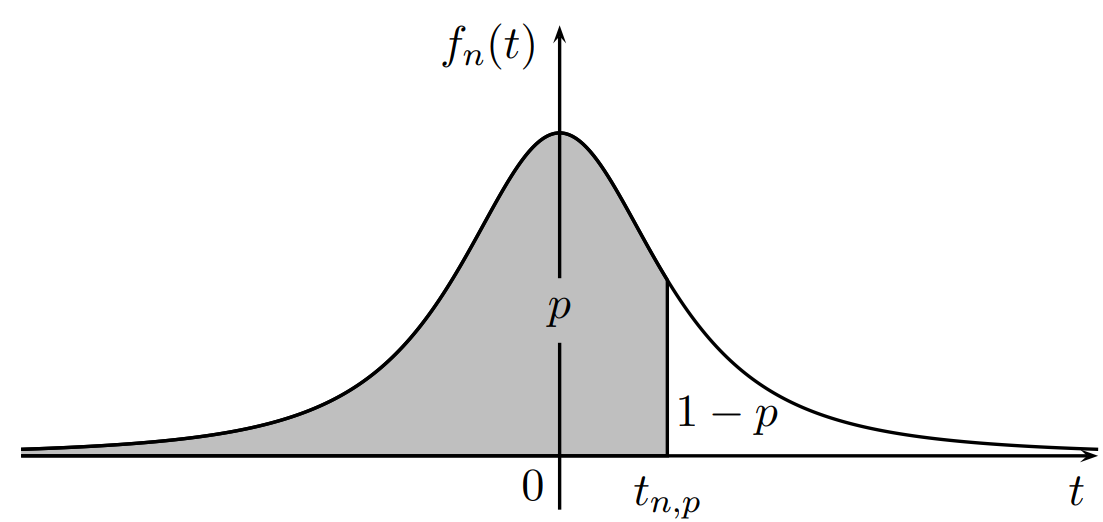
\includegraphics[width=.7\linewidth]{Pics/T.3.img.png}
\end{figure}
$p$-quantile $t_{n,p}$ for Student’s $t$-distribution with $n$ degrees of freedom. The density function is symmetric, therefore $t_{n,1-p} = -t_{n,p}$.
\begin{figure}[H]
  \centering
  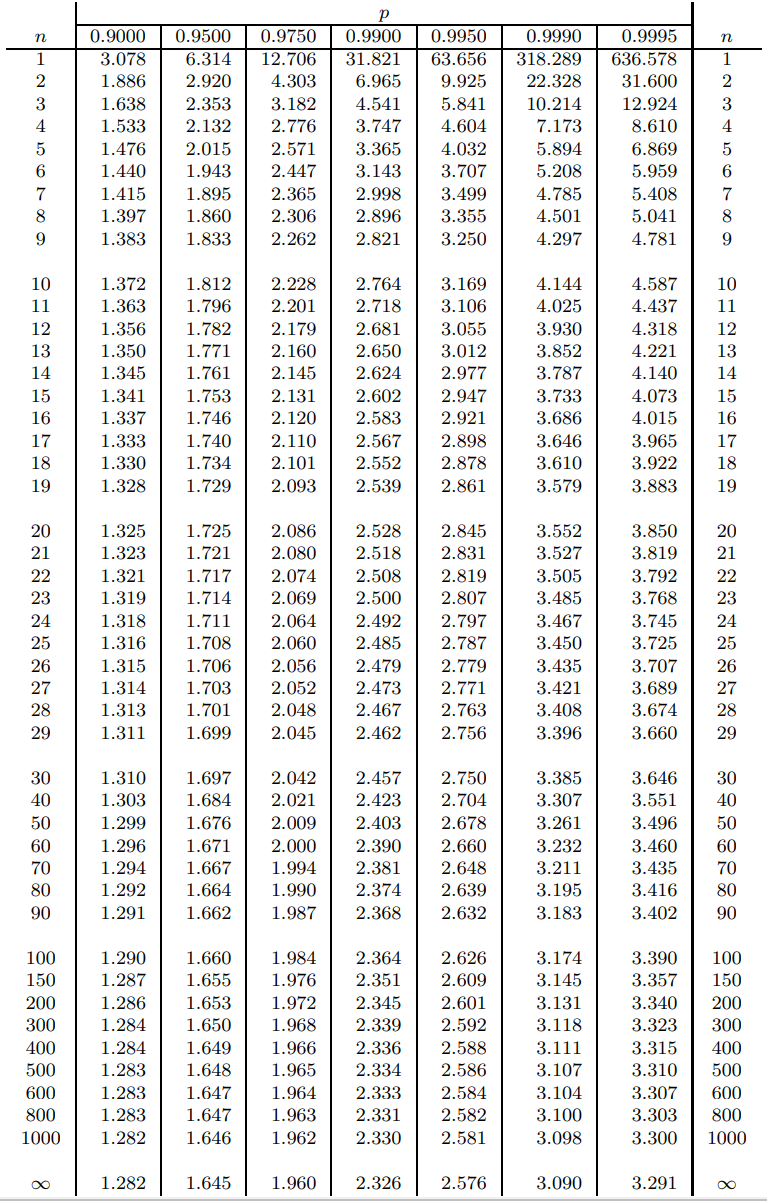
\includegraphics[width=\linewidth]{Pics/T.3.png}
\end{figure}

\section{Factors for constructing control charts}
\noindent\rule[\linienAbstand]{\linewidth}{\linienDickeDick}
\begin{figure}[H]
  \centering
  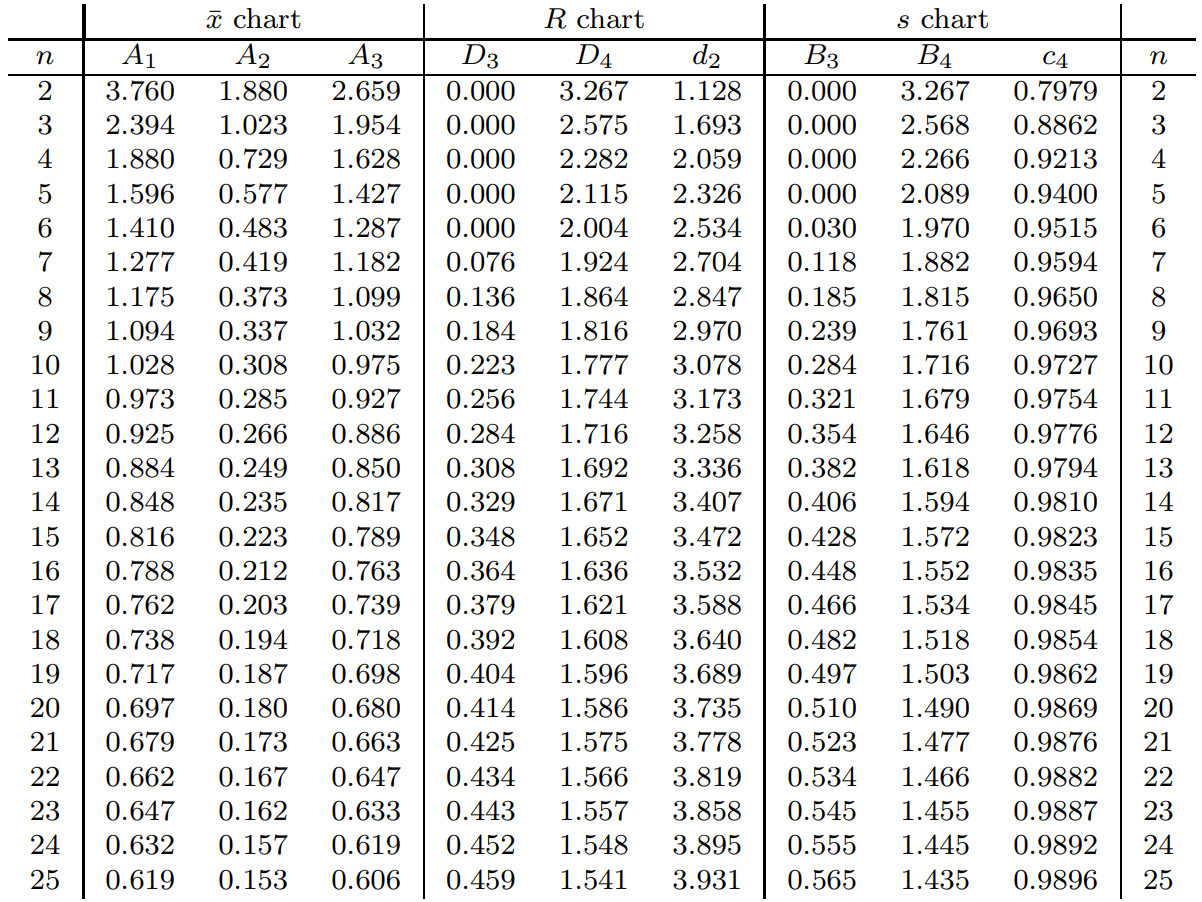
\includegraphics[width=\linewidth]{Pics/T.15.png}
\end{figure}

For the tukey's ascombe plot
what is the assumption?
what should the plot look like if the assumption is true
what do I actually see?
Conclusion?


\end{multicols*}
\end{document}
